\documentclass{book}
\usepackage{physics}
\usepackage{graphicx}
\usepackage{caption}
\usepackage{amsmath}
\usepackage[shortlabels]{enumitem}
\usepackage[left=1in,right=1in,top=1in,bottom=1in]{geometry}
\usepackage{bm}
\usepackage{authblk}
\usepackage{empheq}
\usepackage{amsfonts}
\usepackage{esint}
\usepackage[makeroom]{cancel}
\usepackage{dsfont}
\usepackage{centernot}
\usepackage{mathtools}
\usepackage{bigints}
\usepackage{amsthm}
\theoremstyle{definition}
\newtheorem{defn}{Definition}[section]
\newtheorem{prop}{Proposition}[section]
\newtheorem{rmk}{Remark}[section]
\newtheorem{thm}{Theorem}[section]
\newtheorem{exmp}{Example}[section]
\newtheorem{prob}{Problem}[section]
\newtheorem{sln}{Solution}[section]
\newtheorem*{prob*}{Problem}
\newtheorem{exer}{Exercise}[section]
\newtheorem*{exer*}{Exercise}
\newtheorem*{sln*}{Solution}
\usepackage{empheq}
\usepackage{hyperref}
\usepackage{tensor}
\usepackage{xcolor}
\hypersetup{
	colorlinks,
	linkcolor={black!50!black},
	citecolor={blue!50!black},
	urlcolor={blue!80!black}
}

\newcommand{\diag}{\text{diag}}
\newcommand{\psirot}{\ket{\psi_\text{rot}(t)} }
\newcommand{\RWA}{\ham_\text{rot}^\text{RWA}}


\newcommand{\lambdabar}{{\mkern0.75mu\mathchar '26\mkern -9.75mu\lambda}}



\newcommand*\widefbox[1]{\fbox{\hspace{2em}#1\hspace{2em}}}

\newcommand{\p}{\partial}
\newcommand{\R}{\mathbb{R}}
\newcommand{\C}{\mathbb{C}}
\newcommand{\lag}{\mathcal{L}}
\newcommand{\nn}{\nonumber}
\newcommand{\ham}{\mathcal{H}}
\newcommand{\M}{\mathcal{M}}
\newcommand{\I}{\mathcal{I}}
\newcommand{\K}{\mathcal{K}}
\newcommand{\F}{\mathcal{F}}
\newcommand{\w}{\omega}
\newcommand{\lam}{\lambda}
\newcommand{\al}{\alpha}
\newcommand{\be}{\beta}
\newcommand{\x}{\xi}


\newcommand{\Else}{\text{else}}
\newcommand{\N}{\mathcal{N}}


\newcommand{\sig}{\bm\sigma}
\newcommand{\n}{\mathbf{n}}
\newcommand{\X}{\mathbf{X}}
\newcommand{\s}{\mathbf{S}}

\newcommand{\G}{\mathcal{G}}

\newcommand{\f}[2]{\frac{#1}{#2}}

\newcommand{\ift}{\infty}

\newcommand{\lp}{\left(}
\newcommand{\rp}{\right)}

\newcommand{\lb}{\left[}
\newcommand{\rb}{\right]}

\newcommand{\lc}{\left\{}
\newcommand{\rc}{\right\}}


\newcommand{\V}{\mathbf{V}}
\newcommand{\U}{\mathbf{U}}
\newcommand{\Id}{\mathbb{I}}
\newcommand{\D}{\mathcal{D}}
\newcommand{\Z}{\mathbf{Z}}
\newcommand{\had}{\mathbf{H}}
\newcommand{\Y}{\mathbf{Y}}
%\setcounter{chapter}{-1}


\makeatletter
\renewcommand{\@chapapp}{Chapter}
%\renewcommand\thechapter{$\bf{\ket{\arabic{chapter}}}$}
%\renewcommand\thesection{$\bf{\ket{\arabic{section}}}$}
%\renewcommand\thesubsection{$\bf{\ket{\arabic{subsection}}}$}
%\renewcommand\thesubsubsection{$\bf{\ket{\arabic{subsubsection}}}$}
\makeatother



\usepackage{subfig}
\usepackage{listings}
\captionsetup[lstlisting]{margin=0cm,format=hang,font=small,format=plain,labelfont={bf,up},textfont={it}}
\renewcommand*{\lstlistingname}{Code \textcolor{violet}{\textsl{Mathematica}}}
\definecolor{gris245}{RGB}{245,245,245}
\definecolor{olive}{RGB}{50,140,50}
\definecolor{brun}{RGB}{175,100,80}
\lstset{
	tabsize=4,
	frame=single,
	language=mathematica,
	basicstyle=\scriptsize\ttfamily,
	keywordstyle=\color{black},
	backgroundcolor=\color{gris245},
	commentstyle=\color{gray},
	showstringspaces=false,
	emph={
		r1,
		r2,
		epsilon,epsilon_,
		Newton,Newton_
	},emphstyle={\color{olive}},
	emph={[2]
		L,
		CouleurCourbe,
		PotentielEffectif,
		IdCourbe,
		Courbe
	},emphstyle={[2]\color{blue}},
	emph={[3]r,r_,n,n_},emphstyle={[3]\color{magenta}}
}


\begin{document}
	\begin{titlepage}\centering
		\clearpage
		\title{{\textsc{\textbf{ATOMIC, MOLECULAR, AND OPTICAL PHYSICS}}}\\ \smallskip - A Quick Guide - \\}s
		\author{\bigskip Huan Q. Bui}
		\affil{Massachusetts Institute of Technology}
		\date{\today}
		\maketitle
		\thispagestyle{empty}
	\end{titlepage}

\subsection*{Preface}
\addcontentsline{toc}{subsection}{Preface}

Greetings,\\

This guide is based on 8.421 and 8.422 at MIT, two courses on atomic, molecular, and optical (AMO) physics, taught by Professor Martin Zwierlein between 2022 and 2023. The purpose of this guide is to provide a short summary of the most basic concepts in AMO physics and serve as a reference for PhD qualification exams in this field. This guide may not be treated as a textbook, and the reader may find much more pedagogical resources in the bibliography. Familiarity with undergraduate physics is recommended. \\

\noindent Enjoy! 

\newpage
\tableofcontents
\newpage



%%%%%%%%%%%%%%%%%%%%%%%%%%%%%%%%%%%%%%%%%%%%%%
%%%%%%%%%%%%%%%%%%%%%%%%%%%%%%%%%%%%%%%%%%%%%%



\chapter{Harmonic Oscillators and Resonance}


\section{The Lorentz Oscillator Model}

This model is incredibly powerful and is one of the most fundamental topics to know and understand when learning AMO physics. So let's get started. We will first consider a \textbf{classical harmonic oscillator} first. For non-trivial dynamics, we consider the case where this system is damped and driven. 
\begin{equation}\label{eq:lorentz}
\ddot x + \gamma \dot x + \omega_0^2 x = \f{F_0}{m}\cos(\omega t).
\end{equation}
Here $\gamma,\omega_0,m,F_0$ take their usual meanings. As a review, we shall introduce the general steady-state solution (we typically don't care about transient behavior) and write down the under-damping condition explicitly. To do this, we have to solve the ODE  \eqref{eq:lorentz}. Then, we will answer some questions that will improve our understanding of the model. \\



\noindent \textbf{\underline{What is the general solution?}}  \\


To make the forthcoming algebraic manipulations clearer, let us use complex notations, so that $\cos(\omega t) \to e^{i\omega t}$. Since the problem concerns only the steady-state solution, we shall ignore the transient behavior and consider the following ansatz oscillating at the drive frequency $\omega$:
\begin{align*}
x(t) = A e^{i\omega t } e^{i\phi}
\end{align*}
where $A \in \mathbb{R}$ is the amplitude and $\phi \in \mathbb{R}$ is the phase. Plugging the ansatz into the ODE, we find 
\begin{align*}
x(t) = A e^{i\omega t} e^{i\phi} \implies -A e^{i \omega t + i\phi} \lp \omega^2 -\omega_0^2 - i\gamma \omega \rp = \f{F_0}{m}e^{i\omega t} \implies A = \f{F_0/m}{-\omega^2 + \omega_0^2 + i\gamma \omega} e^{-i\phi}.
\end{align*}
Since $A$ is real, the denominator of $A$ must be a complex number of the form $\abs{A} e^{-i\phi}$ where
\begin{align*}
\abs{A} = \sqrt{{(\omega_0^2 - \omega^2)}^2 + (\gamma \omega)^2}.
\end{align*}
And the phase $\phi$ is\footnote{I should have used $e^{-i\phi}$ so that $\phi$ in this definition would be the phase \textit{lag}... but okay.}
\begin{align*}
\boxed{\phi = -\arctan(\f{\gamma\omega}{\omega_0^2 - \omega^2})}
\end{align*}
With these, we may write
\begin{align*}
\boxed{A = \f{F_0/m}{\sqrt{(\omega_0^2 - \omega^2)^2 + (\gamma \omega)^2}}}
\end{align*}
The oscillator is underdamped, so we want the roots of the associated chacteristic polynomial $\lambda^2 + \gamma \lambda + \omega_0^2 = 0$:
\begin{align*}
\lambda\pm = -\f{\gamma}{2} \pm \f{1}{2}\sqrt{\gamma^2 - 4\omega_0^2}
\end{align*}
to be complex (to get oscillations on top of an exponential decay). As a result, we require that 
\begin{align*}
\gamma^2 < 4\omega_0^2 \iff \boxed{\gamma < 2\omega_0}
\end{align*}
This is the standard underdamping condition. \\


\noindent \textbf{\underline{At which $\omega$ do we get maximal amplitude response?}} \\

Before proceeding, let us introduce two dimensionless quantities $\rho = \omega/\omega_0$ and $f = \gamma/\omega_0$ and rewrite $A$ as 
\begin{align*}
A =  \lp \f{F_0}{m \omega_0^2}\rp \f{1}{\sqrt{(1-\rho^2)^2 + (f\rho)^2}}
\end{align*}
Finding $\omega$ so that $A$ is maximal requires finding $\rho$ for which the denominator of $A$ is minimal:
\begin{align*}
\f{d}{d\rho}\lb (1-\rho^2)^2 + (f\rho)^2 \rb = 2\rho(-2 + f^2 + 2\rho^2).
\end{align*}
Setting the expression above to zero tells us that $\rho$ could be $0$ or $\sqrt{1-f^2/2}$ (we must also verify that $A$ has a global maximum, but I won't go into the details here). Since $f = \gamma/\omega_0 \in (0,2)$ we must consider two cases:
\begin{itemize}
	\item If ${0 < f \leq \sqrt{2}}$ then the solution $\rho = \sqrt{1-f^2/2}$ is real and we have 
	\begin{align*}
	A(0)= \f{F_0}{m\omega_0^2} <  \f{F_0}{m\omega_0^2} \lp \f{2}{f\sqrt{4-f^2}}\rp  = A\lp \sqrt{1-f^2/2}\rp
	\end{align*}
	because $f\sqrt{4-f^2} \leq 2$ for $f\in (0,2)$. We therefore see that $A$ attains its maximum at $$\boxed{\omega = \omega_0 \sqrt{1- \gamma^2/2\omega_0^2}}$$
	
	
	
	\item Otherwise, if ${\sqrt{2} < f < 2}$ then the solution $\rho = \sqrt{1-f^2/2}$ is imaginary and $A$ attains its maximum of $F_0/m\omega_0^2$ at $$\boxed{\omega = 0}$$
\end{itemize}
Contrary to what we might expect, the maximal amplitude is attained \textbf{NOT} at the resonance frequency $\omega_0$. Rather, depending on the ratio $\gamma/\omega_0$, we have different answers. \\



\noindent \textbf{\underline{At which $\omega$ does the phase lag between the response and the drive becomes $\pi/2$?}} \\



The phase \textit{lag} being $\pi/2$ means that $\phi = -\pi/2$, i.e.,
\begin{align*}
\arctan\lp \f{\gamma \omega}{\omega_0^2 - \omega^2} \rp = \f{\pi}{2} \implies \boxed{\omega = \omega_0}
\end{align*}
This means that the resonance condition is better characterized by the $\pi/2$ phase lag of the response relative to the drive, rather than the amplitude attaining its maximal value. \\




\noindent \textbf{\underline{When does the power delivered from the drive to the oscillator become maximal?}} \\

Here, by ``power'' we actually mean the power delivered from the drive averaged over one cycle. The power from the drive is given by $P = dW/dt$ where $dW$ is the work done by the drive over an infinitesimal $dx$ and is thus given by $dW = Fdx$.  Putting everything together we have $P = F(t)x'(t)$. The power delivered from the drive, averaged over one cycle of period $T = 2\pi / \omega$, is therefore
\begin{align*}
\langle P \rangle 
&= \f{\omega}{2\pi}\int_{0}^{2\pi/\omega} F_0 \cos(\omega t) \f{d}{dt} \Re{x(t)} \,dt \\
&= \f{F_0 A \omega}{2\pi}  \int_{0}^{2\pi/\omega} \cos(\omega t)  \f{d}{dt} \cos\lp \omega t + \phi \rp \,dt \\
&= -\f{F_0 A \omega^2}{2\pi}  \int_{0}^{2\pi/\omega} \cos(\omega t) \sin\lp \omega t + \phi \rp \,dt \\
&= -\f{1}{2}F_0 A \omega \sin \phi.
\end{align*} 
Plugging in the expressions for $\phi$ and $\omega$ we find 
\begin{align*}
\boxed{\langle P \rangle = \f{F_0^2 }{2m\gamma}\f{(\gamma\omega)^2}{(\omega_0^2 - \omega^2)^2 + (\gamma \omega)^2}}
\end{align*}
We recognize that $P$ has the form of a Lorentzian (or a Cauchy distribution) with FWHM $\gamma$ which attains the maximum $\langle P \rangle_\text{max} = F_0^2/2m\gamma$ at $\omega = \omega_0$.  \textcolor{blue}{One may also use standard calculus techniques to get this result.} \\



\noindent $\boxed{\textbf{!}}$ It makes sense that the power delivered by the drive to the oscillator, averaged over one cycle, is the same as the power dissipated by the damping, averaged one cycle, since the system is in equilibrium in steady state. This can be verified by repeating the calculation above explicitly, but for the damping force. The work done by drag force is $-m\gamma x'(t)$, from which we find the dissipated power is $P_\text{dis} = Fv = m\gamma v(t)^2$. From here, we have
\begin{align*}
\langle P_\text{dis}\rangle = \f{\omega}{2\pi}m\gamma A^2\int_0^{2\pi/\omega} \lp \f{d}{dt}\cos(\omega t + \phi)\rp^2\,dt = \f{1}{2}m\gamma A^2\omega^2.
\end{align*}
Plugging in the expression for $A$ we find that
\begin{align*}
\langle P_\text{dis}\rangle = \f{F_0^2}{2m\gamma} \f{(\gamma\omega)^2}{(\omega_0^2 - \omega^2)^2 + (\gamma \omega)^2} = \langle P \rangle \,\,\,\checkmark
\end{align*}



\noindent \textbf{\underline{Why does the dissipated power become maximal at that frequency?} } \\


When the drive $F \propto \cos (\omega t)$ is at $\omega = \omega_0$, the position $x(t) \propto \cos(\omega_0 t + \phi)$ of the oscillator has a $-\phi =\pi/2$ phase lag compared to the drive. However, the velocity $x'(t) \propto -\sin(\omega_0 t -\pi/2) = \cos(\omega_0 t)$ is now in phase with the drive. As a result, the drive is always doing positive work, and thus $\langle P \rangle$ is maximal.  \\







\noindent \textbf{\underline{Why does reducing $\gamma$ increase $P$ on resonance?}}\\

In the far off-resonance regime, we may assume that $\abs{\omega_0^2 - \omega^2}\gg \gamma \omega$, so that 
\begin{align*}
\langle P \rangle_\text{far off res.}  \approx   \f{F_0^2}{2m\gamma} \f{(\gamma \omega)^2}{(\omega_0^2 - \omega^2)^2} \propto \gamma,
\end{align*}
so $\langle P \rangle$ varies linearly in $\gamma$ for far off-resonance drive. In the near-resonance regime, we may ignore the term $\omega_0^2 - \omega^2$ in the denominator to find 
\begin{align*}
\langle P \rangle_\text{near res.} \approx \f{F_0}{2m\gamma} \propto \gamma^{-1}.
\end{align*}


As the damping is decreased, the amplitude of the motion increases, thereby increasing the dissipated power on resonance. In the limit of no damping $(\gamma = 0)$, the power dissipated on resonance becomes infinite because the amplitude blows up. The line shape of the response becomes that of a Dirac delta function. \\




\noindent \textbf{\underline{On resonance, what is the steady-state average energy stored and dissipated per cycle?}}\\

Now we have resonant driving, so $\omega = \omega_0$. The steady-state average energy stored in the oscillator is the sum of kinetic and potential energy. 
\begin{align*}
\langle KE\rangle &= \f{\omega_0}{2\pi} \int_0^{2\pi/\omega_0} \f{1}{2}m x'(t)^2\,dt=   \f{F_0^2 }{4m\gamma^2}\\
\langle PE \rangle &= \f{\omega_0}{2\pi}\int_0^{2\pi/\omega_0} \f{1}{2}m \omega_0^2 x(t)^2\,dt  = \f{F_0^2}{4m\gamma^2}
\end{align*}
where we have used $x(t) = (F_0/m\gamma \omega_0) \sin(\omega_0 t)$. From here, the total energy stored in the oscillator is 
\begin{align*}
\boxed{\langle E \rangle = \langle KE \rangle + \langle PE \rangle = \f{F_0^2}{2m\gamma^2}}
\end{align*}
On the other hand, the energy dissipated in one cycle may be calculated by integrating the dissipated power over a cycle $E_\text{lost} = \int P_\text{dis}\,dt$ where $P_\text{dis} = F_\text{damp} v(t)$: 
\begin{align*}
\boxed{E_\text{lost} = \int_0^{2\pi/\omega_0} \gamma m x'(t) x'(t)\,dt = \f{F_0^2 \pi}{m\gamma \omega_0}}
\end{align*}
Take the $2\pi$-adjusted ratio of these two results, we find 
\begin{align*}
2\pi \f{\langle E \rangle}{E_\text{lost}} = \f{\omega_0}{\gamma},
\end{align*}
which is nothing but the \textbf{quality factor} $\boxed{Q = \omega_0 / \gamma}$.\\










\noindent \textbf{\underline{What happens when the mass has charge $q$ and is driven by $F = e\mathcal{E}\cos(\omega t)$?}}\\


This is the \textbf{Lorentz Oscillator Model}. When $\gamma = 0$ (undamped -- we will think about what damping means in this case), the steady-state dipole moment $d(t) = ex(t)$ is given by:
\begin{align*}
d(t) = ex(t) = \f{e^2 E\cos(\omega t)}{\omega_0^2 - \omega^2}.
\end{align*}
This expression is related to a concept called \textbf{oscillator strength} which we will look at later. \\




Even in the absence of other kinds of damping, the motion will be damped because
of what is called \textbf{radiation damping}, $\gamma = \Gamma_{\text{rad}}$. From classical electrodynamics, we know that
any accelerated charge will emit radiation. The total power radiated by an accelerated
electron in the full solid angle of $4\pi$ (see \cite{griffiths2005introduction} for details) is 
\begin{align*}
P = \f{1}{6\pi \epsilon_0 c^3}|\ddot{d}|^2.
\end{align*}



\noindent \textbf{\underline{On resonance, what is the energy lost per orbital cycle?}}\\

Taking the amplitude of $x(t)$ to be $x_0$, the total power radiated in the full solid angle of $4\pi$ is 
\begin{align*}
P = \f{1}{6\pi \epsilon_0 c^3}\abs{\ddot d}^2 = \f{e^2 x_0^2 \omega_0^4 \cos^2(\omega_0 t)}{6 c^3 \pi \epsilon_0}.
\end{align*}
The energy lost per orbital cycle is thus
\begin{align*}
E_\text{lost} = \int_0^{2\pi/\omega_0} P\,dt = \f{e^2 x_0^2 \omega_0^3}{6c^3 \epsilon_0}.
\end{align*}



\noindent \textbf{\underline{From $E_\text{stored}$ and $E_\text{lost}$, what is $\Gamma_\text{rad}$? }}\\

The total energy is calculated in the same manner as before:
\begin{align*}
\langle KE\rangle &= \f{\omega_0}{2\pi} \int_0^{2\pi/\omega_0} \f{1}{2}m x'(t)^2\,dt= \f{1}{4}m \omega_0^2 x_0^2  \\
\langle PE \rangle &= \f{\omega_0}{2\pi}\int_0^{2\pi/\omega_0} \f{1}{2}m \omega_0^2 x(t)^2\,dt  = \f{1}{4}m \omega_0^2 x_0^2 \\
E_\text{stored} &= \langle KE \rangle + \langle PE \rangle = \f{1}{2}m \omega_0^2 x_0^2
\end{align*}
From here, we get
\begin{align*}
Q = 2\pi \f{E_\text{stored}}{E_\text{lost}} = \f{6c^3 m\pi \epsilon_0}{e^2 \omega_0}.
\end{align*}
Since $Q = \omega_0 / \Gamma_{\text{rad}}$, we find
\begin{align*}
\boxed{\Gamma_\text{rad} = \f{\omega_0}{Q} = \f{e^2 \omega_0^2}{6c^3 m \pi \epsilon_0}}
\end{align*} 

\noindent \textbf{\underline{What is $Q$ in terms of the classical radius of the electron and $\lambdabar $ of the emission?}}\\


In terms of the classical radius of the electron
\begin{align*}
r_0 = \f{e^2}{4\pi \epsilon_0 mc^2}, 
\end{align*}
we have
\begin{align*}
Q = \f{3\lambdabar}{2r_0} \quad\quad \text{and}\quad\quad \Gamma_\text{rad} = \f{\omega_0}{Q} = \f{2r_0c}{3\lambdabar^2}
\end{align*}




\noindent \textbf{\underline{Estimate $Q,\Gamma_\text{rad}$ for the Sodium D2 line.}}\\



With $\lambda = 589 $ nm, we have
\begin{align*}
Q &\approx 5.0 \times 10^7 \\
\Gamma_\text{rad} &\approx 2\pi \times 10.2 \text{ MHz}
\end{align*}
which is in remarkable agreement with the experimentally measured natural line width for the D2 line of Na which is $2\pi \times 9.795(11)$ MHz. The calculation is within $\sim 5$\% of the measured value.  





\subsection{The Signal-to-Noise ratio and the quality factor}



Let's look at the expression for the power delivered to the oscillator again:
\begin{align*}
{\langle P \rangle = \f{F_0^2 }{2m\gamma}\f{(\gamma\omega)^2}{(\omega_0^2 - \omega^2)^2 + (\gamma \omega)^2}}
\end{align*}
Near resonance, we may make the following approximation:
\begin{align*}
\omega_0^2 - \omega^2 \approx 2\omega(\omega_0  - \omega),
\end{align*}
so that 
\begin{align*}
\langle P \rangle = \f{F_0^2 }{2m\gamma} \f{1}{1 + \lp \f{\omega - \omega_0}{\gamma/2}\rp ^2}.
\end{align*}
This is a Lorentzian with FWHM $\Delta \omega = \gamma$. The time constant for the decay constant $\gamma$ is simply $\tau = 1/\gamma$. The quality factor is again $Q = \omega_0  / \gamma = \omega_0 / \Delta \omega$. From here, we see that
\begin{align*}
\tau \Delta \omega = 1
\end{align*}
which can be treated as an uncertainty relation, which characterizes \textbf{individual measurements}. This means we can actually find $\omega_0$ to better than $\Delta \omega$ with multiple measurements. To be more precise: In the presence of noise, the frequency precision with which the center can be located, $\delta \omega$, depends on the signal-to-noise ratio via
\begin{align*}
\delta \omega = \f{\Delta \omega}{S/N},
\end{align*}
as a rule of thumb. This means that we can see that with high $S/N$, we can measure $\omega_0$ very precisely. This is what we mean by ``splitting the resonance line.'' Typically, experimenters can split the line by a factor of $10^3$. 


\section{The Quantum Harmonic Oscillator}


Consider a 1D harmonic oscillator of mass $m$ and frequency $\omega$ in a number state $\ket{n}$. \\




\noindent \textbf{\underline{How are the annihilation and creation operators $ a$ and $ a^\dagger$ relate to $ x$ and $ p$?}}\\


Let $a = A  x - i B  p$, where $A,B$ are real scalars, so that $ a^\dagger = A x+ i B  p$. We want the following to hold:
\begin{align*}
\ham = \f{p^2 }{2m} + \f{1}{2}m\omega^2 x^2 = \hbar \omega \lp a^\dagger a + \f{1}{2} \rp
\end{align*}
so we compute
\begin{align*}
\hbar \omega \lp a^\dagger a+ \f{1}{2}\rp = \hbar \omega A^2 x^2 + \hbar \omega B^2 p^2 + \hbar \omega AB + \f{\hbar \omega}{2}
\end{align*}
where we have used $[x,p] = i\hbar $. By setting 
\begin{align*}
A = \sqrt{\f{m\omega}{2\hbar}} \quad\quad B = -\sqrt{\f{1}{2\hbar m\omega}}
\end{align*}
the first equation is satisfied. We therefore conclude that
\begin{align*}
a = \sqrt{\f{m\omega}{2\hbar}} \lp x + \f{i}{m\omega} p \rp \quad\quad a^\dagger = \sqrt{\f{m\omega}{2\hbar}} \lp x - \f{i}{m\omega} p \rp.
\end{align*}
From here, we find 
\begin{align*}
\boxed{x = \sqrt{\f{\hbar}{2 m\omega}}(a^\dagger + a) \quad\quad\text{and}\quad\quad p = i\sqrt{\f{\hbar m\omega }{2}}(a^\dagger - a)}
\end{align*}




\noindent \textbf{\underline{What are the average and rms position and momentum?}}\\


From the results above, we get
\begin{align*}
\bra{n} x \ket{n} = \sqrt{\f{\hbar}{2 m\omega}}\bra{n} a^\dagger + a \ket{n} = 0
\end{align*}
\begin{align*}
\bra{n} p \ket{n} = i\sqrt{\f{\hbar m\omega }{2}}\bra{n} a^\dagger - a \ket{n} = 0
\end{align*}
since both $a^\dagger$ and $a$ respectively send $\ket{n}$ to $\ket{n+1}$ and $\ket{n-1}$ which are orthonormal to $\ket{n}$. Next, 


\begin{align*}
\sqrt{\bra{n}p^2 \ket{n}} &= \sqrt{-\f{\hbar m\omega}{2}\bra{n} (a^\dagger - a)^2 \ket{n} }\\
&= \sqrt{-\f{\hbar m\omega}{2} \bra{n} a^\dagger a^\dagger -a^\dagger a - aa^\dagger + a^2 \ket{n} }\\
&= \sqrt{\hbar m\omega \lp n+ \f{1}{2} \rp}.
\end{align*}

\begin{align*}
\sqrt{\bra{n}x^2 \ket{n}} &= \sqrt{\f{\hbar}{2 m\omega}\bra{n} (a^\dagger + a)^2 \ket{n} }\\
&= \sqrt{\f{\hbar}{2 m\omega}\bra{n} a^\dagger a^\dagger +a^\dagger a + aa^\dagger + a^2 \ket{n} }\\
&= \sqrt{\f{\hbar}{m\omega}\lp n+ \f{1}{2} \rp}.
\end{align*}







\noindent \textbf{\underline{Check the results above using energy and the virial theorem.}}\\



The total energy is 
\begin{align*}
\langle  E\rangle  = \f{\langle p^2\rangle }{2m} + \f{1}{2}m\omega^2 \langle x^2\rangle = \f{1}{2m}\hbar m\omega \lp n+ \f{1}{2} \rp + \f{1}{2}m\omega^2 \f{\hbar}{m\omega}\lp n+ \f{1}{2} \rp  = \hbar \omega\lp n+ \f{1}{2}\rp \,\,\, \checkmark
\end{align*}

Virial theorem: Since $V\propto x^2$, the virial theorem states that $\langle T \rangle  = \langle V \rangle$. From the calculation above, we see that this holds:
\begin{align*}
\langle T \rangle =  \f{1}{2m}\hbar m\omega \lp n+ \f{1}{2} \rp  = \f{1}{2}m\omega^2 \f{\hbar}{m\omega}\lp n+ \f{1}{2} \rp = \langle V \rangle \,\,\, \checkmark
\end{align*}






\noindent \textbf{\underline{What is the rms size and velocity for Na in $\ket{0,0,0}$ with $\omega = 2\pi \times 100$ Hz?}}\\


For a Na atom in the state $\ket{0,0,0}$ of a 3D harmonic potential, we have, by spherical symmetry:
\begin{align*}
\sqrt{\langle r^2\rangle} = \sqrt{3\langle x^2 \rangle } = \sqrt{3(2\cdot 0+1)\f{\hbar}{2m\omega}} = \sqrt{\f{3\hbar}{2m\omega}}.
\end{align*}
With $\omega = 2\pi \times 100 $ Hz and $m_\text{Na} \approx 23 \times 1.66054\times 10^{-27}$ kg, the rms size is
\begin{align*}
\sqrt{\langle r^2\rangle} \approx 2.57 \text{ \textmu m}.
\end{align*}




Similarly, we can find the rms velocity using spherical symmetry:
\begin{align*}
\sqrt{\langle v^2 \rangle} = \f{1}{m}\sqrt{\langle p^2 \rangle} = \f{1}{m}\sqrt{3\langle p_x^2 \rangle} = \f{1}{m}\sqrt{3(2\cdot 0 + 1) \f{\hbar m \omega}{2}} = \sqrt{\f{3\hbar \omega}{2m}}.
\end{align*}
The numerical value for this is
\begin{align*}
\sqrt{\langle v^2 \rangle} \approx 1.61 \text{ mm/s}.
\end{align*}







%%%%%%%%%%%%%%%%%%%%%%%%%%%%%%%%%%%%%%%%%%%%%%
%%%%%%%%%%%%%%%%%%%%%%%%%%%%%%%%%%%%%%%%%%%%%%





\chapter{The Two-Level System}









\section{Magnetic Resonance: Classical Spin in $\mathbf{{B}(t)}$}





\subsection{Classical spin in a magnetic field}

Consider a classical spin in a magnetic field. Let this spin have some angular momentum which we will always write as $\hbar \bm{J}$. The interaction energy is given by 
\begin{align*}
	W = -\bm{\mu} \cdot \cdot \bm{B}.
\end{align*} 
The force acting on the spin is the gradient of this energy function
\begin{align*}
	\bm{F} = -\grad W = \grad (\bm{u}\cdot \bm{B}).
\end{align*}
And the torque on the spin is 
\begin{align*}
	\bm{\tau} = \bm{\mu}\times \bm{B}.
\end{align*}
Here, 
\begin{align*}
	\bm{\mu} = \gamma (\hbar \bm{J})
\end{align*}
stands for the magnetic moment, which is directly related to angular momentum via the \textbf{gyromagnetic ratio $\gamma$}.

Now torque is rate of change of angular momentum, so we have 
\begin{align*}
	\f{d\hbar \bm{J}}{dt} = \bm{\mu}\times \bm{B} \implies \boxed{\f{d\bm{J}}{dt} = \gamma \bm{J}\times \bm{B} = -\gamma \bm{B}\times \bm{J}}
\end{align*}
This says that the motion of $\bm{J}$ is pure precession about $\bm{B}$, where $\bm{J}$ has constant magnitude and tipping angle $\theta$ relative to $\bm{B}$. The rate of precession is determined by the magnetic field strength $B$ and the gyromagnetic ratio $\gamma$:
\begin{align*}
	\Omega_L = -\gamma B.
\end{align*}
This rate of precession is called the \textbf{Larmor frequency}.\\



\noindent \underline{\textbf{Example:}} Consider an electron traveling with velocity $v$ in a circular loop of radius $r$ and area $A = \pi r^2$. We may consider a current $I = dq/dt = e v/2\pi r$ associated with this motion and find the magnetic moment to be $\bm{\mu} = I A \hat{\bm{z}}$. It is easy to see that 
\begin{align*}
	\bm{\mu} = I A \hat{\bm{z}} = \f{evr}{2} \hat{\bm{z}} = \f{e}{2m} mvr \hat{\bm{z}} = \lp \f{e\hbar}{2m} \rp \lp \f{L}{\hbar} \rp \hat{\bm{z}}
\end{align*}
Here, the quantity $e\hbar / 2m$ is the famous \textbf{Bohr magneton}, $\mu_B$. It is important to remember that for electrons, $\gamma_e \approx -2\mu_B$, whereas for classical charge distributions with $L = \hbar$, $\gamma \approx \mu_B$. This discrepancy has to do with the fact that electrons have two spin states, whereas the latter each has 3 spins states, spaced by $\mu_B$.





\subsection{Rotating coordinate transformation}


Consider a vector $\bm{A}$ rotating with angular velocity $\bm{\Omega}$. The equation of motion is 
\begin{align*}
	\f{d}{dt} \bm{A} = \bm{\Omega} \times \bm{A}.
\end{align*}



Now suppose we have a vector  $\bm{A}$ and we go to a system rotating at angular velocity $\bm{\Omega}$ then 
\begin{align*}
	{\lp \f{d\bm{A}}{dt} \rp_\text{inertial} = \lp \f{d\bm{A}}{dt} \rp_\text{rotating} + \bm{\Omega}\times \bm{A}}
\end{align*}
So to go from an inertial to rotating frame we do the following:
\begin{align*}
	\boxed{\lp \f{d}{dt}\cdot \rp_r = \lp \f{d}{dt}\cdot \rp_i - \bm{\Omega}\times \cdot}
\end{align*}
Now consider the vector $\bm{J}$ like before:
\begin{align*}
	\lp \f{d\bm{J}}{dt} \rp_\text{rot}  =  \lp \f{d\bm{J}}{dt} \rp_\text{inertial} - \bm{\Omega}\times \bm{J} = \gamma \bm{B}\times \bm{J} - \bm{\Omega}\times \bm{J} = \gamma \bm{J}\times (\bm{B} + \bm{\Omega}/\gamma)
\end{align*}
If we let 
\begin{align*}
	\bm{B}_\text{eff} = \bm{B} + \bm{\Omega}/\gamma
\end{align*}
then we have a new equation of motion in the frame rotating at $\bm{\Omega}$:
\begin{align*}
	\lp \f{d\bm{J}}{dt} \rp_\text{rot} = \gamma \bm{J} \times \bm{B}_\text{eff}.
\end{align*}
We see that in the rotating frame, $\bm{J}$ precesses about this new effective magnetic field. Notice that $\bm{J}$ is constant in this frame exactly when $\bm{\Omega} = -\gamma \bm{B}$, which is what we saw before.




\subsection{Larmor's Theorem}

The result above is Larmor's Theorem, which states that the effect of a magnetic field on a free charge can be eliminated by a suitable rotating coordinate transformation. \\


Consider a charged particle in a magnetic field $\bm{B}$, under the influence of some applied force $\bm{F}_0$. The total force on the particle is 
\begin{align*}
	\bm{F} = \bm{F}_0 + q\bm{v}\times \bm{B}.
\end{align*}
In a frame rotating at $\bm{\Omega}$, the force is 
\begin{align*}
\bm{F}_{\text{rot}} &= \bm{F} - 2m(\bm{\Omega}\times \bm{v}_\text{rot}) - m\bm{\Omega} \times (\bm{\Omega}\times \bm{r})\\
&= \bm{F}_0 + q\bm{v}\times \bm{B} + 2m\bm{v}\times \bm{\Omega} - m\bm{\Omega}\times (\bm{\Omega}\times \bm{r}).
\end{align*}
from classical mechanics and substitution. Notice that if we take $\bm{B} = B\hat{\bm{z}}$ and choose 
\begin{align*}
	\bm{\Omega} = -(q/2m)\bm{B}
\end{align*}
then 
\begin{align*}
	\bm{F}_\text{rot} = \bm{F}_0 - m\lp \f{qB}{2m} \rp^2 \hat{\bm{z}} \times (\hat{\bm{z}} \times \bm{r}).
\end{align*}
Typically the $B^2$ term is small, so we may drop it to obtain 
\begin{align*}
	\bm{F}_\text{rot} = \bm{F}_0.
\end{align*}
We see that for the case of a charged particle in a magnetic field $B_0$, by going to a rotating frame with $\Omega = qB/2m $, we are able to eliminate the effect of $B_0$.





\subsection{Motion in a rotating magnetic field}

So far we have considered static magnetic fields and transformed between inertial and rotating frames whose angular velocity is dependent on the field strength and the gyromagnetic ratio (remember that $\Omega = \gamma B$). Now, we will consider what happens when the magnetic field itself rotates. \\


The setup is as follows. Consider a magnetic moment $\bm{\mu}$ precessing about a static field $\bm{B}_0 = B_0 \hat{\bm{z}}$. The rate of precession, a.k.a. the Larmor frequency, is $\omega_0 = \gamma B_0$. The motion of the moment is given by 
\begin{align*}
	\mu_z = \mu\cos\theta, \quad \mu_x = \mu\sin\theta \cos\omega_0t, \quad \mu_y = -\mu\sin\theta \sin\omega_0 t.
\end{align*}


Now we introduce an additional magnetic field $\bm{B}_1$ in the $xy$-plane which rotates at a constant angular frequency $\omega$. We consider two cases. \\



\noindent \textbf{Exact resonance:} In this case, $\omega = \omega_0 = \gamma B_0$. In this case, the full magnetic field is 
\begin{align*}
	\bm{B}(t) = B_1(\cos\omega_0 t \,\, \hat{\bm{x}} -\sin\omega_0 t \,\, \hat{\bm{y}}) + B_0 \hat{\bm{z}}
\end{align*}


What is the motion of $\bm{\mu}$? To do this, we go the frame rotating with $\bm{B}_1$. In this frame, the $z$-axis is the same as the inertial frame, and the $xy$-plane rotates with $\bm{B}_1$. It is easy to see that in this frame, the rotating magnetic field is constant. The effective magnetic field in this frame is thus
\begin{align*}
	\bm{B}_\text{eff}(t) 
	&= \bm{B}(t) - (\omega_0/\gamma) \hat{\bm{z}}\\
	&= B_1(\cos\omega_0 t \,\, \hat{\bm{x}} -\sin\omega_0 t \,\, \hat{\bm{y}}) + (B_0 - \omega_0/\gamma) \hat{\bm{z}}\\
	&= B_1 \hat{\bm{x}}'  + (B_0 - \omega_0/\gamma) \hat{\bm{z}}\\
	&= B_1 \hat{\bm{x}}'.
\end{align*}

Notice that all time dependence is removed. In the rotating frame, the magnetic field is static in the $x$-axis and has value $B_1$, the strength of the rotating magnetic field. The motion of the moment in the rotating frame is then very simple: the problem is reduced to that for a moment in a static field. It is clear that the moment, in this rotating frame, precesses around the $B_1 \hat{\bm{x}'}$ field at angular velocity:
\begin{align*}
	\omega_R = \gamma B_1.
\end{align*}
This is called the \textbf{Rabi frequency}. Remember the difference between Larmor and Rabi frequency! If the moment initially points along the positive $z$-axis, then after $t = \pi/\omega_R$, the moment points the negative $z$-axis: it has completely turned over. 

\begin{figure*}[!htb]
	\centering
	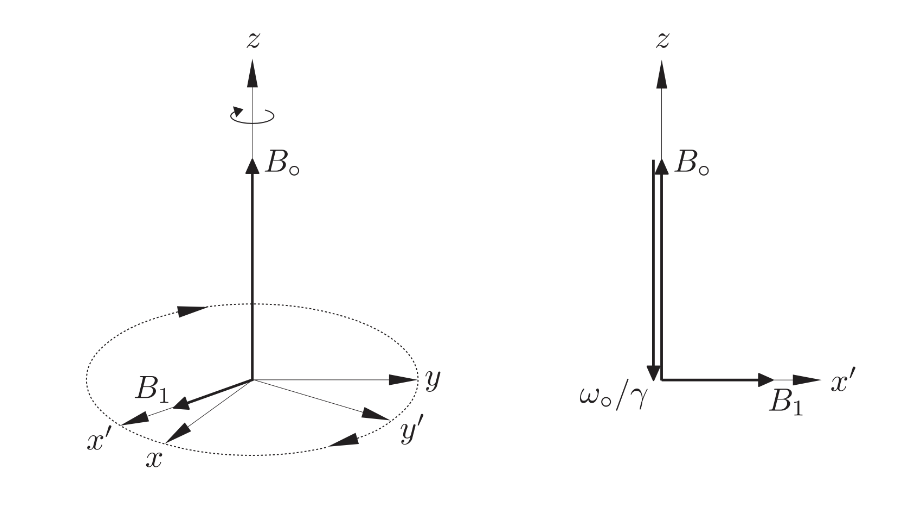
\includegraphics[width=0.7\textwidth]{figures/rotatingB.png}
\end{figure*}


In the inertial frame, the motion of the moment is a combination of precession around the $\hat{\bm{x}}'$ axis (at Rabi frequency $\omega_R = \gamma B_1$) and the rotation of $\hat{\bm{x}}'$ around the $z$-axis (at rate $\omega = \gamma B_0$). 


 




\noindent \textbf{Off-resonant behavior:}  In this case, the rotating magnetic field rotates at a rate $\omega \neq \omega_0 = \gamma B_0$, and therefore:
\begin{align*}
	\bm{B}_\text{eff}(t) = B_1 \hat{\bm{x}}' + (B_0 - \omega_0/\gamma) \hat{\bm{z}}.
\end{align*}

There is still no time dependence, so the effective magnetic field is still static. However, this field makes an angle $\theta$ with the $z$-axis. Since the field is static, we also know that the moment (in the rotating frame) precesses about it, at a rate given by the gyromagnetic ratio $\gamma$ multiplied by the strength of the effective field: 
\begin{align*}
	\boxed{\Omega_R = \gamma B_\text{eff} = \gamma \sqrt{(B_0 - \omega/\gamma)^2 + B_1^2} = \sqrt{(\omega_0 - \omega)^2 + \omega_R^2}}
\end{align*}
This quantity is called the \textbf{generalized Rabi frequency}.\\


Suppose the moment points along the positive $z$-axis like before. What, then, is its motion? The motion of its $x$-component is more complicated and less relevant so we will ignore that. Motivated by quantum mechanics, we will only care about its $z$-component. Finding $\mu_z(t)$ is a simple geometry problem. The answer is 
\begin{align*}
	\boxed{\mu_z(t) = \mu\lb 1 - 2\f{\omega_R^2}{\Omega_R^2}\sin^2 \f{\Omega_R t}{2} \rb}
\end{align*}
Notice that $\mu_z(t)$ never completely flips sign unless $\omega = \omega_0$. It turns out that the quantum mechanical result (which we will soon find) is identical. 




\subsection{Rapid Adiabatic Passage: Landau-Zener Crossing}

Rapid adiabatic passage is a technique for spin-flipping a population by sweeping through resonance. This ``sweeping through resonance'' is achieved when the frequency of the oscillating field ($\omega$) or the transition frequency ($\omega_0$) is \textit{slowly} varied. \\


The problem is essentially solved in view of the last two subsections, so here we present a qualitative solution to strengthen our intuition. Consider the setup as before, with the exception that the rotating field $\bm{B}_1$ initially rotates slowly and far from resonance $\omega \ll \omega_0 = \gamma B_0$. In the rotating frame, the effective magnetic field $\bm{B}_\text{eff}$ is approximately the field in the inertial frame, but without rotation. The magnetic moment precesses about $\bm{B}_\text{eff}$, making a tight angle with it (Here we assume that the moment is initially aligned with the $z$-axis). \\

Now, if we slowly sweep $\omega$ through resonance ($\omega_0$), the magnetic moment will continue to precess tightly around $\bm{B}_\text{eff}$ and will follow it adiabatically.  Eventually, when $\omega \gg \omega_0  = \gamma B_0$, the magnetic moment will be inverted. 


\begin{figure*}[!htb]
	\centering
	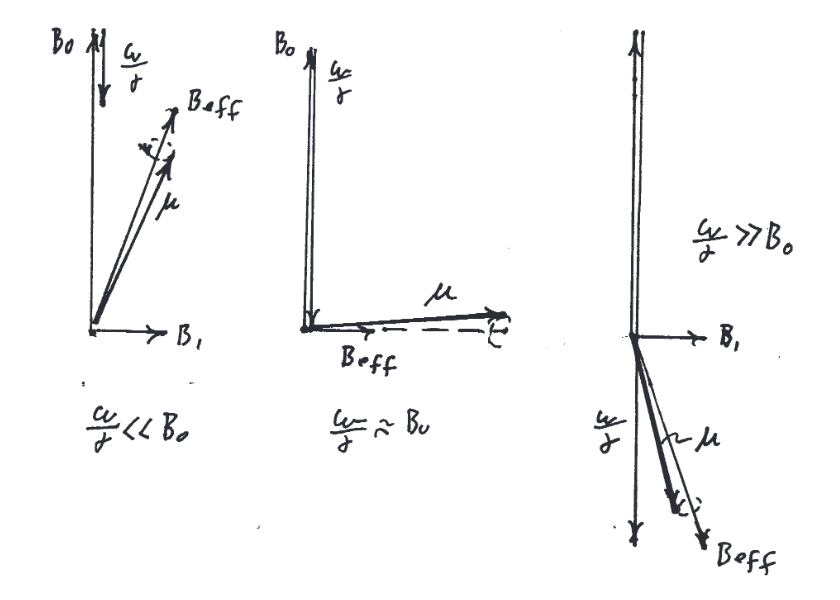
\includegraphics[width=0.75\textwidth]{figures/LZ_following}
\end{figure*}


How slow is \textit{slow}? In order for this adiabatic following to happen, we must require that within one precession period $2\pi/\Omega_R$, the angle that $\bm{B}_\text{eff}$ makes with the $z$-axis must not have advanced by more than a few degrees (Remember that in the expression $B_\text{eff} = B_0 - \omega/\gamma$, the rotation rate $\omega$ is changing.) So, we must have that
\begin{align*}
	\Delta \theta = \dot{\theta} \cdot \Delta t = \dot \theta \f{2\pi}{\Omega_R}  \ll 2\pi \implies \dot \theta \ll \Omega_R,
\end{align*}
i.e., the generalized Rabi frequency $\Omega_R$ must be large compared to the rate at which $\bm{B}_\text{eff}$ is changing direction. Since $B_\text{eff}(t)= B_0 - \omega(t)/\gamma$, and the fact that this requirement is most severe near exact resonance where $\omega = \omega_0 \implies \theta = \pi/2$. So we want:
\begin{align*}
	\f{1}{\gamma B_1} \f{d\omega}{dt} \ll \omega_R.
\end{align*}
But since $\omega_R = \gamma B_1$, the condition is 
\begin{align*}
	\boxed{\dot{\omega} \ll \omega_R^2}
\end{align*}
To summarize, in order for rapid adiabatic passage to occur, we want to slowly sweep from far off-resonance through resonance. To do this, we have to compare $\omega$ to $\omega_0$ and $\dot \omega$ to $\omega_R^2$ and make sure the conditions above hold. \\




A few things to notice. First, the argument above applies for the case where we sweep $\omega$ from above ($\gg \omega_0$) to below ($\ll \omega_0$). Second, rapid adiabatic passage is generally \textit{slower} than a spin-flip using an on-resonance $\pi$-pulse. This is because $\dot \omega$ must be small compared to $\omega_R^2$ (and thus $\omega_R$). 


\subsection{Adiabatic Following in a Magnetic Trap}


As an aside, LZ-crossing explains atom-losses in magneto-optical traps. This happens when an atom traverses through the zero-field region in the MOT. As it does, the rate of change of the field becomes infinitely large, and the atoms fails to follow the field adiabatically and undergoes a spin flip which removes it from the trap. The size of this region is dictated by the speed of the atom $v$ and the gyromagnetic ratio $\gamma$, and the field gradient $B'$:
\begin{align*}
	r = \sqrt{\f{v}{\gamma B'}}.
\end{align*}
This region is also called the \textbf{Majorana hole}.









\section{Resonance of a Quantized Spin}




\subsection{Expectation value of magnetic moment behaves classically}


Now we treat this problem quantum mechanically. First, we will show that the expectation value of magnetic moment behaves classically, i.e. 
\begin{align*}
	\f{d}{dt}\langle \hat{\bm{\mu}} \rangle = \gamma \langle \hat{\bm{\mu}}\rangle \times \bm{B}.
\end{align*}

To do this, we recall the Heisenberg equations of motion for an operator $\hat{O}$:
\begin{align*}
	\f{d}{dt}\hat{O} = \f{i}{\hbar}[\hat{H}, \hat{O}] + \f{\p}{\p t}\hat{O}.
\end{align*}

The Hamiltonian of $\hat{\bm{\mu}}$ interacting with a magnetic field $\bm{B}_0  B_0 \hat{\bm{z}}$ is
\begin{align*}
	\hat{H} = -\hat{\bm{\mu}} \times \bm{B}_0 = -\gamma B_0 \hat{J}_z.
\end{align*}
Using the definition $\hat{\bm{\mu}} = \gamma \hat{\bm{J}}$ and commutation rules, one finds that 
\begin{align*}
	\f{d}{dt}\hat{J}_x = \gamma B_0 \hat{J}_y, \quad\quad \f{d}{dt}\hat{J}_y = -\gamma B_0 \hat{J}_x, \quad\quad \f{d}{dt}\hat{J}_z = 0.
\end{align*}
In particular, by taking expectation values, we find 
\begin{align*}
	\f{d}{dt}\langle \hat{\bm{\mu}} \rangle = \gamma \langle \hat{\bm{\mu}}\rangle \times \bm{B}.
\end{align*}


We see that the quantum mechanical and classical equation of motion are identical. A few more things:
\begin{itemize}
	\item This result is valid for any angular momentum operator, and thus is valid for spin-1/2.
	
	\item It is therefore valid for any system that can be mapped onto an effective spin-1/2.
	
	\item It is valid for the case of several angular momenta within an atom coupled to a total angular momentum $\bm{F}$ (so long as the magnetic field is not large enough to break the coupling)
	
	\item It is valid also for a system of $N$ two-level systems symmetrically coupled to an external field. 
\end{itemize} 


\subsection{The Rabi Problem}


In this subsection we provide the full quantum mechanical treatment of the quantized spin in a magnetic field problem. We will then compare our results to the classical treatment seen earlier. \\


To this end, we first write down the Hamiltonian for this system. The magnetic moment is $\bm{\mu} = \gamma \hbar \bm{S}$. It is placed in a uniform magnetic field $\bm{B}_0 = \omega_0 \hat{\bm{z}} /\gamma$, where $\omega_0 = \omega_2 - \omega_1$. Starting at $t=0$, $\bm{B}_R(t)$ rotates in the $xy$-plane with frequency $\omega$. The Hamiltonian is 
\begin{align*}
	H = -\bm{\mu}\cdot \bm{B} = -\bm{\mu}\cdot (\bm{B}_0 + \bm{B}_R(t)).
\end{align*}
By decomposing each term into its $x,y,z$-components, we obtain 
\begin{align*}
	H = \hbar
	\begin{pmatrix}
		\omega_1 & \omega_R e^{i\omega t}/2 \\
		\omega_R e^{-i\omega t}/2 & \omega_2 
	\end{pmatrix}.
\end{align*}
Alternatively, we could consider this problem with the rotating field being oscillatory in only one direction $x$ or $y$. In this case, the Hamiltonian is just a linear superposition of the $x$- and $y$-Hamiltonians. We will focus on the case where the field is along $\hat{\bm{x}}$. \\

\noindent  \textbf{Solution:} The Hamitonian of the system in the Schr\"{o}dinger picture is 
	\begin{align*}
		\ham_S(t) &= \hbar \begin{pmatrix}
			\omega_1 & \omega_R \cos \omega t \\ \omega_R \cos\omega t & \omega_2
		\end{pmatrix} \\
		&= \f{\hbar}{2} \begin{pmatrix}
			2\omega_1 & \omega_R (e^{-i\omega t} + e^{i\omega t}) \\ \omega_R (e^{-i\omega t} + e^{i\omega t}) & 2\omega_2
		\end{pmatrix}.
	\end{align*}
	where we chosen a basis where $\ket{1} = (1 \,\,\, 0)^\top$ and $\ket{2} = (0 \,\,\, 1)^\top$ and used the fact that the coupling between state $\ket{2}$ and state $\ket{1}$ is $\hbar \omega_R \cos\omega t$. Let us go to rotating frame via the operator
	\begin{align*}
		T = e^{i\sigma_z \omega t/2} = \begin{pmatrix}
			e^{i\omega t/2} &  0 \\0  & e^{-i\omega t/2}
		\end{pmatrix} 
	\end{align*}
	whose purpose is to transform our system such that the new Hamiltonian associated with the transformed system is time-independent\footnote{I'm explicitly avoiding the language "$T$ transforms the original Hamiltonian into a time-independent Hamiltonian" because we actually don't have $\ham_\text{rot} = T^\dagger \ham_S T$.}.  We have the following relations between the rest frame and rotating frame:
	\begin{align*}
		\text{States: } \ket{\psi_\text{rot}(t)} = T^\dagger \ket{\psi(t)} \quad\quad \text{Operators: }  A_\text{rot}(t) = T^\dagger A(t) T.
	\end{align*}
	
	The Schr\"{o}dinger equation in the rotating frame can be obtained from the Schr\"{o}dinger equation in the rest frame. From
	\begin{align*}
		i\hbar \f{d}{dt}\ket{\psi(t)} 
		&= i\hbar \f{d}{dt}\lp T\psirot \rp \\
		&= i\hbar \dot T \psirot + i\hbar T \f{d}{dt}\psirot\\
		&= \ham_S(t)\ket{\psi(t)} \\
		&= \ham_S(t) T\psirot
	\end{align*}
	we deduce that $\psirot$ satisfies the equation
	\begin{align*}
		i\hbar \f{d}{dt}\psirot = \lp T^\dagger \ham_S(t) T -i\hbar T^\dagger \dot T \rp \psirot.
	\end{align*} 
	With this we may define the rotating frame Hamiltonian:
	\begin{align*}
		\ham_\text{rot}(t) = T^\dagger \ham_S(t) T -i\hbar T^\dagger \dot T
	\end{align*}
	so that
	\begin{align*}
		i\hbar \f{d}{dt}\psirot = \ham_\text{rot}(t) \psirot.
	\end{align*}


	Now we simplify the problem by using the  \textbf{rotating frame approximation} (RWA).  The steps are as follows: we first transform the original Hamiltonian into the interaction picture, make the RWA, then transform the Hamiltonian back, and then go to the rotating frame. \\
	
	The original Hamiltonian may be decomposed into a field-free part and a perturbation part: 
	\begin{align*}
		\ham(t) = \ham_0 + \ham_1(t) = \hbar \begin{pmatrix}
			\omega_1 & 0 \\ 0 & \omega_2
		\end{pmatrix} + \f{\hbar}{2} \begin{pmatrix}
			0 & \omega_R (e^{-i\omega t} + e^{i\omega t}) \\ \omega_R (e^{-i\omega t} + e^{i\omega t}) & 0
		\end{pmatrix}.
	\end{align*}
	The interaction Hamiltonian is then 
	\begin{align*}
		\ham_{1,I}(t) = e^{i\ham_0 t/\hbar} \ham_{1}(t) e^{-i\ham_0 t/\hbar} = 
		\f{\hbar\omega_R}{2}\begin{pmatrix}
			0 & e^{-i(\omega + \omega_0)t} + e^{+i(\omega - \omega_0)t}   
			\\ 
			e^{+i(\omega + \omega_0)t} + e^{-i(\omega - \omega_0)t} & 0
		\end{pmatrix}
	\end{align*}
	where we have defined $\omega_0 = \omega_2 - \omega_1$. Here, we observe that since the drive is near resonance, the $e^{\pm it(\omega - \omega_0)}$ terms vary very slowly compared to the rapidly oscillating $e^{\pm it(\omega+\omega_0)}$ terms. Therefore, we may approximate $\ham_{1,I}(t)$ by dropping the latter:
	\begin{align*}
		\ham_{1,I}^{\text{RWA}}(t) = \f{\hbar\omega_R}{2}\begin{pmatrix}
			0 & e^{+i(\omega - \omega_0)t}   
			\\ 
			e^{-i(\omega - \omega_0)t} & 0
		\end{pmatrix}
	\end{align*}
	Transforming back to the Schr\"{o}dinger picture, we find:
	\begin{align*}
		\ham_S^\text{RWA}(t) = \ham_0 + e^{-i\ham_0 t/\hbar} \ham_{1,I}^{\text{RWA}}(t) e^{+i\ham_0 t/\hbar} = \f{\hbar}{2}\begin{pmatrix}
			2\omega_1 & \omega_R e^{i\omega t} \\ \omega_R e^{-i\omega t} & 2\omega_2
		\end{pmatrix}.
	\end{align*}
	Finally, to proceed with the problem, let us to go rotating frame:
	\begin{align*}
		\boxed{\ham_\text{rot}^\text{RWA}} &= T^\dagger \ham_S^\text{RWA}(t) T -i\hbar T^\dagger \dot T \\
		&= \boxed{\f{\hbar}{2} \begin{pmatrix}
				\omega + 2 \omega_1 & \omega_R \\ \omega_R & - \omega + 2\omega_2
		\end{pmatrix}}
	\end{align*}

	\textbf{This is a very important Hamiltonian to remember.} If there's anything to take away from solving this problem, it is to remember that we first have a Hamiltonian in the Schr\"{o}dinger picture. We then make the rotating wave approximation by first transforming the Hamiltonian into the interaction picture (where is it decomposed into the "bear" part and "interaction" part), make the RWA, and then transform back into the Schr\"{o}dinger picture. Next, we go to the rotating frame. The rest of the problem is linear algebra on the Hamiltonian we just found. \\
	
	
	
	Mathematica code:
	\begin{lstlisting}
		(*define H1*)
		In[3]:= H1 = (h/2)*{{0, 
				wR*(E^(-I*w*t) + E^(I*w*t))}, {wR*(E^(+I*w*t) + E^(-I*w*t)), 0}};
		
		(*define H0*)
		In[4]:= H0 = h*{{w1, 0}, {0, w2}};
		
		(*H1 in interaction picture*)
		In[34]:= H1I = 
		TrigToExp[MatrixExp[I*H0*t/h] . H1 . MatrixExp[-I*H0*t/h]];
		
		(*H1 in RWA, back to Schrodinger picture*)
		In[25]:= H1RWA = (h*wR/2)*
		TrigToExp[
		MatrixExp[-I*H0*t/h] . {{0, 
				E^(+I*t*(w - (w2 - w1)))}, {E^(-I*t*(w - (w2 - w1))), 0}} . 
		MatrixExp[+I*H0*t/h]] // FullSimplify;
		
		(*New Schrodinger Hamiltonian after RWA*)
		In[33]:= HRWA = H1RWA + H0;
		
		(*Rotating frame transformation T*)
		In[28]:= T = MatrixExp[I*PauliMatrix[3]*w*t/2];
		
		(*full Hamiltonian, after RWA and going into rotating frame*)
		In[32]:= HRWArot = 
		FullSimplify[
		ConjugateTranspose[T] . HRWA . T - 
		I*h*ConjugateTranspose[T] . D[T, t], Assumptions -> {w > 0, t > 0}]
		
		(*result!*)
		Out[32]= {{1/2 h (w + 2 w1), (h wR)/2}, {(h wR)/2, h (-(w/2) + w2)}}
	\end{lstlisting}
	
	
	
	
	
	
	
	
	
	
	Now, let us make the following symmetrization. Let $\omega_\text{avg} = (\omega_1 + \omega_2)/2$ and $\omega_0 = \omega_2 - \omega_1$, then we have
	\begin{align*}
		\RWA = \f{\hbar}{2} \begin{pmatrix}
			\omega +  2\omega_1 & \omega_R \\ 
			\omega_R  & -\omega + 2\omega_2
		\end{pmatrix}
		= 
		\f{\hbar}{2} \begin{pmatrix}
			\omega -  \omega_0 & \omega_R \\ 
			\omega_R  & -\omega +\omega_0 
		\end{pmatrix}
		+ \hbar \begin{pmatrix}
			\omega_\text{avg} & 0 \\ 0 & \omega_\text{avg}
		\end{pmatrix}.
	\end{align*}
	Let us go a step further and define the \textbf{detuning} $\delta = \omega - \omega_0$ to get
	\begin{align*}
		\boxed{\RWA = \f{\hbar}{2}\begin{pmatrix}
			\delta & \omega_R \\  \omega_R & -\delta
		\end{pmatrix} + \hbar \omega_\text{avg} \mathbb{I}}
	\end{align*}
	\textbf{This is the same as before, but in a more compact and easy-to-remember form.} The eigenvalues of this Hamiltonian are
	\begin{align*}
		E_\pm \pm \f{\hbar}{2}\sqrt{\delta^2 + \omega_R^2} + \hbar \omega_\text{avg} = \pm \f{\hbar \Omega_R}{2} + \hbar \omega_\text{avg}
	\end{align*}
	where we have defined the generalized Rabi frequency $\Omega_R = \sqrt{\delta^2 + \omega_R^2}$. To get eigenvectors, we solve the system 
	\begin{align*}
		\RWA \begin{pmatrix}
			c_1 \\ c_2
		\end{pmatrix} = E_\pm \begin{pmatrix}
			c_1 \\ c_2
		\end{pmatrix}
	\end{align*}	
	under the normalization condition $\abs{c_1}^2 + \abs{c_2}^2 = 1$. By inspection, we must have that
	\begin{align*}
		c_2 &=  \f{E_\pm - \hbar \omega_\text{avg} - \hbar \delta/2}{\hbar \omega_R/2} c_1 \\
		&\implies \lb 1 + \lp \f{2E_\pm}{\hbar \omega_R}  - \f{2\omega_\text{avg}}{\omega_R} - \f{\delta}{\omega_R}\rp^2 \rb \abs{c_1}^2 = \lb 1 + \lp  \f{\pm \sqrt{\delta^2+\omega_R^2}}{\omega_R} - \f{\delta}{\omega_R}\rp^2 \rb \abs{c_1}^2 = 1
	\end{align*}
	Let us call $\cos\phi = \delta/\Omega_R$ and $\sin\phi = \omega_R / \Omega_R$. For $E_+$, we can simplify:
	\begin{align*}
		1 = \abs{c_1}^2 \lb 1+ \lp \f{1}{\sin\phi} - \cot\phi \rp^2 \rb = \f{1}{\cos^2(\phi/2)} \implies c_1 = \cos\f{\phi}{2} \implies c_2 = \sin\f{\phi}{2}.
	\end{align*}
	We can do the same for $E_-$ and get
	\begin{align*}
		&c_1 = +\cos\f{\phi}{2} \implies c_2 = \sin\f{\phi}{2} \quad\quad\text{for } E_+\\
		&c_1 = -\sin\f{\phi}{2} \implies c_2 = \cos\f{\phi}{2} \quad\quad\text{for } E_-
	\end{align*}
	from which we can express the eigenvectors in terms of the stationary basis vectors $\ket{1}$ and $\ket{2}$:
	\begin{align*}
		&\ket{+_\text{rot}(t)} = +\cos \f{\phi}{2} \ket{1} + \sin\f{\phi}{2}\ket{2} \\
		&\ket{-_\text{rot}(t)} = -\sin \f{\phi}{2} \ket{1} + \cos\f{\phi}{2}\ket{2}
	\end{align*}
	where we have arbitrarily picked a phase to get "nice" results. This lets us write the wavefunction in the rotating frame at $t=0$ as 
	\begin{align*}
		\ket{\psi_\text{rot}(0)} = \ket{\psi(0)} = \ket{1} = \cos\f{\phi}{2}\ket{+_\text{rot}(t)} -\sin\f{\phi}{2}\ket{-_\text{rot}(t)},
	\end{align*}
	from which we can derive its time evolution (also in the rotating frame):
	\begin{align*}
		\psirot 
		&= e^{-i \RWA t/\hbar} \ket{\psi_\text{rot}(0)} \\
		&= \cos\f{\phi}{2}e^{-i E_+ t/\hbar} \ket{+_\text{rot}(t)} -\sin\f{\phi}{2}e^{-i E_- t/\hbar}\ket{-_\text{rot}(t)}\\
		&= e^{-i\omega_\text{avg} t}\lb \cos\f{\phi}{2} e^{-i\Omega_R t/2} \ket{+_\text{rot}(t)} - \sin\f{\phi}{2}e^{+i\Omega_R t/2} \ket{-_\text{rot}(t)} \rb\\
		&= e^{-i\omega_\text{avg} t}\lb \cos\f{\phi}{2} e^{-i\Omega_R t/2} \textcolor{blue}{\lp \cos \f{\phi}{2} \ket{1} + \sin\f{\phi}{2}\ket{2} \rp}- \sin\f{\phi}{2}e^{+i\Omega_R t/2} \textcolor{blue}{\lp -\sin \f{\phi}{2} \ket{1} + \cos\f{\phi}{2}\ket{2}  \rp } \rb \\
		&= e^{-i\omega_\text{avg} t}\lb \lp \cos^2\f{\phi}{2} e^{-i\Omega_R t/2}+\sin^2\f{\phi}{2} e^{i\Omega_R t/2}  \rp \ket{1} + \lp e^{-i\Omega_R t/2} - e^{i\Omega_R t/2}  \rp \cos\f{\phi}{2}\sin\f{\phi}{2}\ket{2} \rb \\
		&= e^{-i\omega_\text{avg} t}\lb \lp \cos\f{\Omega_R t}{2} - i\cos \phi \sin\f{\Omega_R t}{2} \rp \ket{1} - i\sin\phi \sin\f{\Omega_R t}{2} \ket{2} \rb \\
		&= e^{-i\omega_\text{avg}t }\lb \lp \cos\f{\Omega_R t}{2} - i\f{\delta}{\Omega_R} \sin\f{\Omega_R t}{2}   \rp \ket{1} - i\f{\omega_R}{\Omega_R} \sin\f{\Omega_R t}{2} \ket{2}\rb.
	\end{align*}
	
	To obtain the wavefunction $\ket{\psi(t_1)}$ in the lab frame we have to transform it back via
	\begin{align*}
		\ket{\psi(t_1)} &= T \ket{\psi_\text{rot}(t_1)}\\
		&= \boxed{e^{-i\omega_\text{avg}t_1 }\lb e^{i\omega t_1/2} \lp \cos\f{\Omega_R t_1}{2} - i\f{\delta}{\Omega_R} \sin\f{\Omega_R t_1}{2}   \rp \ket{1} - i e^{-i\omega t_1/2}\f{\omega_R}{\Omega_R} \sin\f{\Omega_R t_1}{2} \ket{2}\rb}
	\end{align*}
	
	
	
	
	
	
	
	
	 
	
	
	The probability of finding the system in state $\ket{2}$ at time $t_1$ is 
	\begin{align*}
		\boxed{P_2(t_1) = \abs{\bra{2}\ket{\psi_\text{rot}(t_1)}}^2 = \f{\omega_R^2}{\Omega_R^2}\sin^2 \lp \f{\Omega_R t_1}{2} \rp}
	\end{align*}
	\textbf{Notice that this is exactly like the classical result we have seen before!}\\
	
	
	
	Suppose we wish to evolve the lab frame wavefunction, then
	\begin{align*}
		\ket{\psi(t)} = e^{-i\omega_\text{avg}t }\lb e^{i\omega t/2} \lp \cos\f{\Omega_R t}{2} - i\f{\delta}{\Omega_R} \sin\f{\Omega_R t}{2}   \rp \ket{1} - i e^{-i\omega t/2}\f{\omega_R}{\Omega_R} \sin\f{\Omega_R t}{2} \ket{2}\rb.
	\end{align*}
	under the field-free, time-independent Hamiltonian 
	\begin{align*}
		\ham_\text{free} = \hbar \begin{pmatrix}
			\omega_1 & 0 \\ 0 & \omega_2
		\end{pmatrix}.
	\end{align*}
	It is clear that with the associated unitary time evolution operator
	\begin{align*}
		U(t) = e^{-i \ham_\text{free} t /\hbar} 
	\end{align*}
	we have, for $t > t_1$,
	\begin{align*}
		\boxed{\ket{\psi(t > t_1)} = e^{-i\omega_\text{avg}t }\lb e^{-i\omega_1 t} e^{i\omega t/2} \lp \cos\f{\Omega_R t}{2} - i\f{\delta}{\Omega_R} \sin\f{\Omega_R t}{2}   \rp \ket{1} - i e^{-i\omega_2 t} e^{-i\omega t/2}\f{\omega_R}{\Omega_R} \sin\f{\Omega_R t}{2} \ket{2}\rb}
	\end{align*}





\subsection{Rapid Adiabatic Passage (Landau-Zener) in a QM treatment}

The Landau-Zener problem for a two-state system or equivalently a spin-1/2 system can be solved rigorously. However, for the sake of understanding we won't worry about the mathematical details here and focus only on the result. \\


Consider a spin-1/2 system in a magnetic field $\bm{B}_\text{eff}$ with energies $W_\pm = \pm \hbar \gamma B_\text{eff}/2$. In a uniform field $B_0$, the effective magnetic field in the rotating frame is simply $B_0 - \omega/\gamma$, where $\omega$ is the rotation rate of the (now zero) magnetic field $B_1$. So in this case, the energies are $W_\pm = \pm \gamma \hbar (B_0 - \omega/\gamma)/2 = \hbar(\omega_0 - \omega)/2$.\\


When $B_1 \neq 0$, as $\omega$ is swept through resonance, the two states move along their changing energies but do not cross (unlike the $B_1 = 0$ case where they do at $\omega = \omega_0$). The states actually follow two hyperbolas separated by an energy $\hbar \omega_R$. If the system moves along these hyperbolas, a spin up will adiabatically convert into a spin down and vice versa. 


\begin{figure*}[!htb]
	\centering
	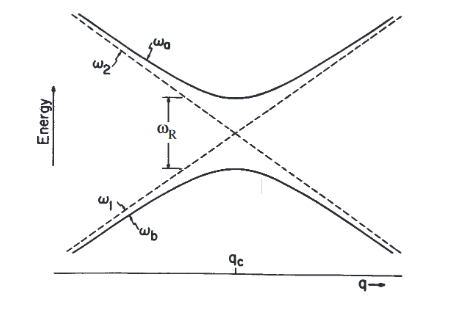
\includegraphics[width=0.5\textwidth]{figures/LZ}
\end{figure*}


Whether the system follows an energy level adiabatically depends on how rapidly the energy is changed relative to the minimum energy separation. It turns out that the probability that the system will \textit{jump} from one adiabatic level to the other after passing through the \textit{avoided crossing} is 
\begin{align*}
	\boxed{P_{na} = \exp\lb - \f{\pi}{2} \f{\omega_R^2}{ d\omega/dt} \rb}
\end{align*}

We see that if we sweep very quickly, then the probability that the spin remains the same is high. Once again, the adiabatic condition we saw before appears here explicitly: For LZ to work as typically desired, we want the sweep rate to be small compared to the Rabi frequency: $\dot \omega \ll \omega_R^2$.





\section{Density Matrix Formalism}


In this section we will outline only some basic results. Given a state $\ket{\psi(t)} = \sum c_n(t) \ket{\psi_n}$, the \textit{density operator} associated with this (pure) state is 
\begin{align*}
	\rho(t) = \ket{\psi(t)} \bra{\psi(t)},
\end{align*}
where its matrix elements are
\begin{align*}
	\rho_{nm}(t) = c_m^*(t) c_n(t). 
\end{align*}

Given some operator $A$, then its matrix elements are $A_{nm} = \bra{\psi_n} A \ket{\psi_m}$. Its expectation at time $t$ is 
\begin{align*}
	\langle A \rangle_t = \bra{\psi(t)} A \ket{\psi(t)}. 
\end{align*}

It is clear, then, that
\begin{align*}
	\langle A \rangle_t = \sum_{nm} \rho_{nm}A_{mn} = \Tr[\rho(t) A]
\end{align*}

So, the density operator allows for easy evaluation of expectation values. \\

States evolve in time, and so do density operators. Applying the SE for the states, we find that the time evolution of density operators is given by the von Neumann equation:
\begin{align*}
	i\hbar \dot \rho = [H,\rho].
\end{align*}


For normalized systems, $\Tr[\rho] = 1$. However, the purity of the system, given by $\Tr[\rho^2]$, is not necessarily unity:
\begin{align*}
	\Tr[\rho^2] \leq \Tr[\rho] = 1.
\end{align*}

$\rho$ is a more general way to represent quantum states since it does not only represent pure states but also statistical ensemble of systems similarly prepared. 

For a two-level system, the density operator has the form
\begin{align*}
	\rho = \begin{pmatrix}
		\rho_{11} & \rho_{12} \\ \rho_{21} & \rho_{22}
	\end{pmatrix}.
\end{align*}
Generically, on-diagonal entries are called \textit{population}, while the off-diagonal entries are called \textit{coherences}. In practice, associated with these quantities are time constants representing their decay. $T_1$ and $T_2$ respectively denote these times. \\

\noindent \textbf{Example:} We may parameterize the Hamiltonian
\begin{align*}
	\ham = -\vec{\mu} \cdot \vec{B} = \f{\hbar}{2}\begin{pmatrix}
		\omega_0 & \omega_R e^{-i\omega t} \\ \omega_R e^{i\omega t} & -\omega_0
	\end{pmatrix}
\end{align*}
in terms of the Pauli matrices as 
\begin{align*}
	\ham = \f{\hbar}{2}\lp 
	\omega_R \cos(\omega t) \, \hat \sigma_x + 
	\omega_R \sin(\omega t) \, \hat \sigma_y + 
	\omega_0 \, \hat\sigma_z \rp.
\end{align*}
In view of the von Neumann equation, we have
\begin{align*}
	i\hbar \dot \rho &= \f{i\hbar}{2} (\dot r_x \,\hat\sigma_x + \dot r_y \,\hat\sigma_y + \dot r_z \,\hat\sigma_z ) \\
	&= [\ham, \rho] \\
	&= \f{\hbar}{4}[\omega_R \cos(\omega t) \, \hat \sigma_x + 
	\omega_R \sin(\omega t) \, \hat \sigma_y + 
	\omega_0 \, \hat\sigma_z , r_x\,\hat\sigma_x + r_y \, \hat \sigma_y + r_z \, \hat \sigma_z].
\end{align*}
where we have used the fact that $\rho = (\mathbb{I} + \vec{r}\cdot \vec{\sigma})/2$. By calculating each $\hat \sigma_i$ term in the commutator, we can find three differential equations for $\vec{r}$, each associated with a component $r_i$. Using the fact that
\begin{align*}
	[\sigma_i, \sigma_j] = 2i \epsilon_{ijk} \sigma_k
\end{align*}
we immediately find the following three equations:
\begin{align*}
	\hat \sigma_x : &\quad\quad \dot r_x = \omega_R \sin(\omega t) r_z - \omega_0 r_y \\
	\hat \sigma_y : &\quad\quad \dot r_y = \omega_0 r_x - \omega_R \cos(\omega t) r_z \\
	\hat \sigma_z : &\quad\quad \dot r_z = \omega_R \cos(\omega t) r_y - \omega_R \sin(\omega t) r_x
\end{align*}
If we now call
\begin{align*}
	\vec{\Omega} = (\Omega_x, \Omega_y, \Omega_z)  =(\omega_R \cos(\omega t), \omega_R \sin(\omega t), \omega_0)^\top
\end{align*}
then it is clear that
\begin{align*}
	\dot r_i = \epsilon_{ijk} \Omega_j r_k.
\end{align*}
In other words, 
\begin{align*}
	\f{d\vec{r}}{dt} = \vec{\Omega} \times \vec{r},
\end{align*}
as desired. This is a nice result which states that the motion of the \textbf{Bloch vector} $\vec{r}$ for a generic two-level system whose Hamiltonian takes the form $\ham = - \vec{\Omega} \cdot \vec{B}$ is given by $d\vec{r}/dt = \vec{\Omega}\times \vec{r}$ where $\abs{\vec{r}}$ is a constant and $\vec{r}$ precesses about $\vec{\Omega}$. Through this particular example we also see that the motion of the Bloch vector for a two-level system subjected to some off-diagonal perturbation corresponds exactly to that of a classical magnetic moment in a magnetic field. \\


Notice further that we have made no assumption about the purity of the system. The fact that $\abs{\vec{r}}$ remains constant in time implies that the purity $\Tr(\rho^2) = (1 + \abs{\vec{r}}^2)/2$ is also constant, i.e. unitary (Hamiltonian) time evolution preserves the purity. In the special case where $\rho$ describes a pure state, we see  that the system remains a pure state. 











\section{Atomic Units}



Units in AMO physics could be \textit{weird} and difficult to familiarize oneself with. These things take some time to get used to and are really only important when one needs to be careful (like doing some meticulous calculation or writing a paper). Personally I like to stick to SI units as much as possible, but Gaussian units could be neat too sometimes. \\





\noindent \textbf{Example:}

\begin{enumerate}[label=\alph*)]
	\item Given $E_A = e/a_0^2$, the energy of the electrostatic potential is given by 
	\begin{align*}
		\mathcal{E}_\text{stat} = \f{e}{a_0^2}  (e a_0) = \f{e^2}{a_0}.
	\end{align*}
	The energy due to quantum confinement may be assumed to be the kinetic energy of the electron, which comes from an angular momentum of $\sim \hbar$, and so 
	\begin{align*}
		\mathcal{E} \sim m_ev^2 = m_e \lp \f{L}{m_ea_0}\rp^2 = \f{\hbar^2}{m_e a_0^2}.
	\end{align*}
	Equating these two energies we find 
	\begin{align*}
		a_0 = \f{\hbar^2}{m_e e^2} \quad\quad \text{in Gaussian units.}
	\end{align*}
	For comparison, the SI-unit definition for the Bohr radius is 
	\begin{align*}
		a_0 = \f{4\pi \epsilon_0\hbar^2}{ m_e  e^2},
	\end{align*} 
	which we would get if we were using SI units. 
	
	\item Suppose that we have an electron is orbiting a proton in a circle of radius $a_0$. We may treat this as a current and calculate the magnetic field produced at the center. Biot-Savart law says that
	\begin{align*}
		dB = \f{\mu_0 I d\vec{l}\times \vec{r}}{4\pi r^2} = \f{\mu_0 I }{4\pi a_0^2}\,dl
	\end{align*}
	for this particular geometry. Here the current $I$ may be computed via
	\begin{align*}
		I = \f{e}{\tau} = \f{e v}{2\pi a_0} = \f{e}{2\pi a_0} \f{\hbar}{m_ea_0} = \f{e \hbar }{2\pi m_ea_0^2}
	\end{align*}
	where we have assumed once again that the electron has angular momentum $L = \hbar =  m_eva_0$. Plugging $I$ into the preceding equation and integrate over the electron orbit we find that, in SI units,
	\begin{align*}
		B_N^{SI} = \oint dB = 2\pi a_0 \f{\mu_0 }{4\pi a_0^2}\f{e \hbar }{2\pi m_e a_0^2} = {\f{\mu_0 e \hbar}{4\pi m_e a_0^3}}
	\end{align*}
	We can now write $B_N^{SI}$ in terms of $E_A^{SI}$:
	\begin{align*}
		B_N^{SI} = \f{\mu_0 e \hbar}{4\pi m_e a_0^3} = \f{\mu_0}{4\pi} \f{\hbar}{m_e} \f{m_e e^2}{4\pi \epsilon_0 \hbar^2}  \f{e}{ a_0^2}  = \f{\mu_0}{4\pi} \f{e^2}{\hbar} E_A^{SI} = \f{\mu_0}{4\pi} \al c 4\pi \epsilon_0 E_A^{SI} = \boxed{\f{\al}{c}E_A^{SI}}
	\end{align*}
	where we have used $1/c = \sqrt{\mu_0 \epsilon_0}$.
	
	
	
	\item Working in SI units, the interaction energy between a Bohr magneton and a magnetic field $B_H$ is given by 
	\begin{align*}
		\mathcal{E} = \mu_B B^{SI}_H = \f{e \hbar}{2 m_e} B_H^{SI}.
	\end{align*}
	The Hartree is given by 
	\begin{align*}
		\mathcal{E}_H = \f{\hbar^2}{m_e a_0^2}.
	\end{align*}
	Setting $\mathcal{E}_H = \mathcal{E}$ gives
	\begin{align*}
		B_H^{SI} = \f{\hbar^2}{m_ea_0^2} \f{2m_e}{e\hbar} = 2\lp \f{\hbar}{e^2} \rp \f{e}{a_0^2} = \f{2}{c}\lp \f{4\pi \epsilon_0 \hbar c}{e^2} \rp \lp \f{e}{4\pi \epsilon_0 a_0^2} \rp = \f{2}{c\al} E_A^{SI} \to \boxed{\f{1}{c\al} E_A^{SI}}
	\end{align*} 
	where we have used $\al = e^2/4\pi \epsilon_0 \hbar c$, the definition of the fine structure constant in SI units, and ignored the factor of 2 as instructed. 
	
	
	\item From Part (c) we have
	\begin{align*}
		B_H^{SI} =  \f{1}{c\al} E_A^{SI} 
	\end{align*}
	To convert this into Gaussian units we invoke the following rules: $B^{SI}_N/B^G_N = \sqrt{\mu_0/4\pi}$ and $E_A^{SI}/E^G_A = 1/\sqrt{4\pi\epsilon_0}$, which give
	\begin{align*}
		\boxed{B_H^{G}} = \sqrt{\f{4\pi}{\mu_0}} \f{1}{c\al} \f{1}{\sqrt{4\pi \epsilon_0}} E_A^{G} = \boxed{\f{1}{\al} E_A^G}
	\end{align*}
	where we have used $1/c = \sqrt{\mu_0 \epsilon_0}$.
	
	
	Similarly we can work out what $B_N^{G}$ is in terms of $E_A^{G}$:
	\begin{align*}
		\boxed{B^G_{N}}= \sqrt{\f{4\pi}{\mu_0}} \f{\al}{c}E_A^{SI} = \sqrt{\f{4\pi}{\mu_0}} \f{\al}{c} \f{1}{\sqrt{4\pi \epsilon_0}} E_A^G = \boxed{\al E_A^G}
	\end{align*}
	In both case we have also used the fact that the (dimensionless) fine-structure constant $\al$ has the same numerical value in SI and Gaussian units.
	
	
	
	\item At first glance we see that $B_N^G \sim \al^2 B_H^G$, so $B_N^G$ is much smaller compared to $B_H^G$. A quick calculation in WolframAlpha gives us 
	\begin{align*}
		B_N^{SI} \approx 12.5\, \text{T} = 125 \, \text{kG}
	\end{align*}
	whereas 
	\begin{align*}
		B_H^{SI} \approx 235 \, \text{kT} = 2.35 \, \text{GG}.
	\end{align*}
	We see that it makes more sense to use $B_N$ as an atomic unit for magnetic fields, as it is closer (in numerical value) to relevant field strengths that we have in the lab (for MOT/BEC/Feshbach resonances, etc.).
\end{enumerate}







%%%%%%%%%%%%%%%%%%%%%%%%%%%%%%%%%%%%%%%%%%%%%%
%%%%%%%%%%%%%%%%%%%%%%%%%%%%%%%%%%%%%%%%%%%%%%


\chapter{The Basics of an Atom}


Our treatment of this chapter will be brief, as its content is better provided by standard quantum mechanics textbooks. 


\section{Spectrosopic notation}

I will assume the reader is familiar with this. 



\section{Hydrogen \& One-electron atoms}

Bohr postulates: 
\begin{itemize}
	\item Electrons protons are point charges whose interaction is coulombic at all distances
	\item Electrons move in circular orbit about the center of mass in stationary states with orbital angular momentum $L = n\hbar$.
	\item One quantum of radiation is emitted when the system changes between these energy levels. From here and basic physics, one finds the energy levels for hydrogen:
	\begin{align*}
		E_n = -\f{1}{2n^2}\lb \f{m}{h^2} \f{e^2}{(4\pi \epsilon_0)^2} \f{M}{m+M} \rb = -\f{hcR_H}{n^2}.
	\end{align*}
	\item The wave number of the radiation is given by the Bohr frequency criterion
	\begin{align*}
		\sigma_{n\to m} = (E_n - E_m)/hc.
	\end{align*}
\end{itemize}

In this part, it is most important to remember that $E \sim 13.6 \text{ eV}/n^2 $ where $n$ is the principal quantum number. For heavier atoms, there an extra factor of $Z^2$, where $Z$ is the number of protons minus the number of inner electrons.\\



\subsection{The Sch\"{o}dinger equation}

I will skip most the build-up in this section and jump directly to important results to remember: In trying to solve for the wavefunctions of hydrogen, one invokes separation of variables, which introduces 3 quantum numbers $n,l,m$.
\begin{align*}
	\psi_{nlm}(\vec{r}) = R_{nl}(r) Y_{lm}(\theta,\phi).
\end{align*} 
Here $R(r)$ is the radial wavefunction, and $Y(\theta,\phi)$ is the radial wavefunction.\\


More specifically, $Y_{lm}(\theta,\phi)$ are spherical harmonics, with $l$ being the eigenvalue of the operator for the orbital angular momentum $\bm{L}$:
\begin{align*}
	\boxed{L^2 Y_{lm} = l(l+1) \hbar^2 Y_{lm}}
\end{align*}
and $m$ is the eigenvalue of the operator for the $z$-projection of the angular momentum operator $L_z$:
\begin{align*}
	\boxed{L_z Y_{lm} = m\hbar Y_{lm}}
\end{align*} 

While we will not write down the differential equation for the radial part here, it is important to remember that in order to simplify it we define the \textit{reduced radial wavefunction} via 
\begin{align*}
	\boxed{R_{nl} = \f{y_{nl}}{r}}
\end{align*} 
From which the original radial equation turns into a new radial equation with an effective radial potential:
\begin{align*}
	\boxed{V_\text{eff}(r) = V(r) + \f{\hbar^2 l(l+1)}{2\mu r^2}}
\end{align*}
where $\mu$ is the reduced mass factor and $V(r)$ is the original radial potential. The second term here is sometimes called the centrifugal potential. This terms adds to the actual potential the kinetic energy of the circular motion that must be present to conserve angular momentum. \\

It is nice to remember that generically, hydrogen-like atoms have wavefunctions of the form
\begin{align*}
	\psi_{nlm} \sim r^l e^{-Zr/na_0} f\lp \f{Zr}{na_0} \rp
\end{align*}
where $a_0$ is the Bohr radius. \\


Also remember that for a given $n$, we have $l = \{0,1,2,\dots, n-1\}$. We require that $l<n$ because no bound state exists for $l \geq n$. In addition, we have that $m = \{ -l,-l+1,\dots, l-1,l \}$.


\subsection{Expectation values of $\langle 1/r^k\rangle$ for hydrogen wavefunctions}

The process for solving for the radial wavefunctions of hydrogen can be found in many intro-to-quantum mechanics textbooks, so we will not worry about it here. However, it is important to remember a few scaling rules for expectation values of $1/r^k$ for the hydrogen wavefunction, as these quantities are often related to other relevant AMO quantities. \\

$k=0$ is the trivial case because that is just the normalization of the wavefunction. \\

For $k=1$, we use the Virial theorem, 
\begin{align*}
	\bigg\langle \f{a_0}{r}\bigg\rangle = \f{1}{n^2}.
\end{align*}
Here, the LHS is related to the potential energy.\\

For $k \geq 2$, we use Feynman-Hellmann theorem, which states that
\begin{align*}
	\f{dE(\lambda)}{d\lambda} = \bra{\psi(\lambda)} \f{dH(\lambda)}{d\lambda} \ket{\psi(\lambda)},
\end{align*}
where $E(\lambda)$ and $\psi(\lambda)$ are the eigenvalue and eigenstate of $H(\lambda)$, respectively. It turns out that
\begin{align*}
	\bigg\langle \f{1}{r^2} \bigg\rangle =   \f{1}{(l+1/2) n^3 a_0^2}
\end{align*}

It also turns out that there is a recursion relation for generating $\langle 1/r^k\rangle$, but only the first couple of outputs are relevant. For $k=3$:
\begin{align*}
	\bigg\langle \f{a_0^3}{n^3} \bigg\rangle &=  \f{1}{l(l+1/2)(l+1) n^3}.
\end{align*}

One more scaling rule: for hydrogenic atoms,
\begin{align*}
	\boxed{\abs{\psi_{n00}(0)}^2 \sim \lp \f{Z}{a_0 n} \rp^3}
\end{align*}


\subsection{Quantum defects}

We won't worry about this, but just to summarize: Consider a hydrogenic atom. We may ask how $E_n$ scales to lowest order. The answer is 
\begin{align*}
	E_n \sim \f{Z^2}{(n-\delta)^2}
\end{align*}
or equivalently, 
\begin{align*}
	E_n  = \f{Z^2R}{n^2} + 2R\f{\delta}{n^3} + \dots 
\end{align*}
for small $\delta$, which is called the \textit{quantum defect}. Here $Z$ is the number of protons minus the number of inner electrons. \\


How does one derive this? The answer is perturbation theory. Suppose that the Hamiltonian for this atom is the usual hydrogen Hamiltonian plus a perturbative part. 
\begin{align*}
	H = H_0 + H',
\end{align*}
where $H'$ is relevant for \textbf{stuff localized near the nucleus}. As a result, the energy shift is 
\begin{align*}
	\Delta E = \bra{\psi_{nl}} H' \ket{\psi_{nl}} \sim \abs{\psi_{nlm}(0)}^2 \sim \f{1}{n^3} \implies \Delta E = 2R\f{\delta}{n^3}
\end{align*}


\section{Some exercises:}

\noindent \textbf{1. Determination of the fine structure constant, $\al$}


\begin{enumerate}[label=(\alph*)]
	\item Our goal is to write $\al$ in terms of $f_\infty = cR_\infty$ and $f_e = m_ec^2/h$. This can be done using the definitions. From $\al =e^2/4\pi \epsilon_0 \hbar c$ we find 
	\begin{align*}
		\al^2 = \f{e^4}{(4\pi \epsilon_0)^2 \hbar^2 c^2} = \f{1}{c^2} f_\infty \f{4\pi \hbar}{m_e} = f_\infty \f{2h}{m_ec^2} = \f{2f_\infty}{f_e}
	\end{align*} 
	where we have used the definition:
	\begin{align*}
		f_\infty = c R_\infty = c\f{m_ee^4}{8 \epsilon_0^2 h^3 c }  =\f{m_ee^4}{8 \epsilon_0^2 h^3 } = \f{m_ee^4}{(4\pi\epsilon_0 \hbar )^2 4\pi \hbar }.
	\end{align*}
	So, 
	\begin{align*}
		\boxed{\al = \sqrt{\f{2f_\infty}{f_e} }}
	\end{align*}
	From here, we see that 
	\begin{align*}
		\al = \sqrt{\f{2cR_\infty}{m_e c^2/h}}
	\end{align*}
	which depends only on the experimental values $R_\infty$ and $h/m_e$. The speed of light $c$ is \textit{defined}. 
	
	
	
	
	\item The de Broglie wavelength for a neutron beam of velocity $v$ is 
	\begin{align*}
		\lambda = \f{h}{m_n v}. 
	\end{align*}
	Therefore we see that by measuring $v$ and $\lambda$ we can measure the ratio $h/m_n$. 
	
	\item The momentum that an atom attains when absorbing a photon of frequency $\nu$ can be derived from conservation of momentum: 
	\begin{align*}
		mv_R = \f{h\nu}{c} \implies \f{h}{m} = \f{cv_R}{\nu}.
	\end{align*}
	
	\item Let's say that an atom absorbs a photon and gets a velocity $v_R$. Assuming that we are working in the non-relativistic limit, the atom sees oppositely Doppler-shifted $\nu_2$ and $\nu_1$:
	\begin{align*}
		&\nu_2' = \nu_2 \lp 1 + \f{v_R}{c} \rp\\
		&\nu_1' = \nu_1 \lp 1 - \f{v_R}{c} \rp
	\end{align*}
	Since we want $\nu_2' = \nu_1'$ which is on resonance with the atoms, we find that
	\begin{align*}
		v_R = c\lp \f{\nu_1- \nu_2}{\nu_1 + \nu_2}\rp.
	\end{align*}
	In the limit where $v_R \ll c$, we may take $\nu = \nu_1 \approx \nu_2$, so that $v_R = h\nu / mc$ and 
	\begin{align*}
		v_R = \f{h\nu}{mc} = \f{c}{2\nu}\Delta \nu \implies \Delta \nu = \f{2h\nu^2}{mc^2} \implies \Delta \omega = \f{2\hbar k^2}{m} \implies \boxed{\f{\hbar}{m} = \f{\Delta \omega}{2k^2}}
	\end{align*}
	where $\nu = \omega/2\pi$ and $k = \omega/c$.
	
	
	
	
	\item By conservation of energy, we must have, for the $m \to m' + \gamma$ transition,
	\begin{align*}
		mc^2 = m'c^2 + pc \implies p = \f{h}{\lambda} = c \Delta m  \implies \boxed{\f{h}{\Delta m} = c\lambda}
	\end{align*}
	where $p$ is the momentum of the photon and $m'<m$. 
\end{enumerate}



\noindent \textbf{2. Ground state energy of the helium atom.}


\begin{enumerate}[label=(\alph*)]
	\item Suppose that both electrons are in the 1s state and that the spin wavefunction is anti-symmetric, then the two-electron spatial wavefunction is the product of the single-electron (normalized) wavefunctions $\psi_{100}(\vec{r})$:
	\begin{align*}
		\Psi(\vec{r}_1, \vec{r}_2) 
		&= \psi_{100}(\vec{r}_1)\psi_{100}(\vec{2})\\
		&= \lb \f{1}{\sqrt{\pi}} \lp \f{Z_\text{He}}{a_0} \rp^{3/2}  e^{-Z_\text{He} r_1/a_0}\rb 
		\lb \f{1}{\sqrt{\pi}} \lp \f{Z_\text{He}}{a_0} \rp^{3/2}  e^{-Z_\text{He} r_2/a_0} \rb\\
		&= \f{1}{\pi} \lp \f{Z_\text{He}}{a_0} \rp^3 e^{-Z_\text{He}(r_1 + r_2)/a_0}.
	\end{align*}
	With this, we may calculate the interaction energy $\langle e^2/r_{12}\rangle$ as follows: 
	\begin{align*}
		\bigg\langle \f{e^2}{r_{12}}\bigg\rangle 
		&= \f{1}{\pi^2}\lp \f{2}{a_0} \rp^6 \int d\phi_1 d\theta_1 dr_1    d\phi_2 d\theta_2 dr_2 \, r_1^2\sin\theta_1  r_2^2\sin\theta_2 \, \f{1}{\abs{\vec{r}_1 - \vec{r}_2}}\exp\lb \f{-4 (r_1 + r_2)}{a_0} \rb.
	\end{align*}
	This is rather complicated, so we make the following simplification. Since we only care about the difference $\vec{r}_1 - \vec{r}_2$, we may take $\vec{r}_1$ to be the $\hat z$-axis for the $\vec{r}_2$ integration. As we integrate through $\vec{r}_1$, this $\hat{z}$-axis will change, but the variables $\theta_1,\phi_1$ will simply integrate out. The point is that with this logic we may take
	\begin{align*}
		\abs{\vec{r}_1 - \vec{r}_2} = \sqrt{r_1^2 + r_2^2 - 2r_1r_2\cos(\theta_2)} 
	\end{align*}
	rather than a complicated formula for the distance between two points in spherical coordinates (which involves all angles $\theta_1,\theta_2,\phi_1,\phi_2$ -- I won't show the full formula here, but it can be derived by going back to Cartesian coordinates). In any case, the integral can be rewritten and evaluated in Mathematica (or by hand if the problem-solver is feeling adventurous):
	\begin{align*}
		\bigg\langle \f{e^2}{r_{12}}\bigg\rangle 
		= \f{1}{\pi^2}\lp \f{2}{a_0} \rp^6  \int_{\mathbb{R}^3} d\phi_1 d\theta_1 dr_1 r_1^2\sin\theta_1  \int_{\mathbb{R}^3}   \, 
		\f{d\phi_2 d\theta_2 dr_2 r_2^2\sin\theta_2}{\sqrt{r_1^2 + r_2^2 - 2r_1r_2\cos(\theta_2)}}\exp\lb \f{-4 (r_1 + r_2)}{a_0} \rb
		= \boxed{\f{5e^2}{4a_0}}
	\end{align*}  
	
	What is this energy in eV? Working in SI units, the energy is given by 
	\begin{align*}
		\bigg\langle \f{e^2}{r_{12}}\bigg\rangle = \f{1}{4\pi \epsilon_0} \lp \f{5e^2}{4a_0} \rp \approx 34.014 \text{ eV}. 
	\end{align*}
	The ground state energy is therefore 
	\begin{align*}
		E_g = -108.848 \text{ eV} + 34.014 \text{ eV} = \boxed{-74.831 \text{ eV}}
	\end{align*}
	which is much closer to the measured value of $-79.006 \text{ eV}$.
	
	
	
	
	
	
	
	
	
	Mathematica code:
	\begin{lstlisting}
		(*define \psi_total^2*)
		In[1]:= f = (1/Sqrt[Pi])*(2/a0)^(3/2)*
		Exp[-2 r1/a0]*(1/Sqrt[Pi])*(2/a0)^(3/2)*Exp[-2 r2/a0]
		
		Out[1]= (8 E^(-((2 r1)/a0) - (2 r2)/a0))/(a0^3 \[Pi])
		
		(*Evaluate integral*)
		In[2]:= e^2*
		Integrate[
		f^2*1/Sqrt[r1^2 + r2^2 - 2 r1*r2*Cos[t2]]*r2^2*Sin[t2]*r1^2*
		Sin[t1], {r1, 0, Infinity}, {r2, 0, Infinity}, {t1, 0, Pi}, {t2, 0,
			Pi}, {p1, 0, 2*Pi}, {p2, 0, 2*Pi}]
		
		Out[2]= ConditionalExpression[(5 e^2)/(4 a0), Re[a0] > 0]
	\end{lstlisting}
	
	
	
	
	
	\item Let us now use variational method to obtain the ground state energy for helium, assuming only the interaction energy $\langle e^2/r_{12}\rangle$ is present. To this end, let us take the trial wavefunction:
	\begin{align*}
		\psi(\vec{r}_1, \vec{r}_2) = \phi(\vec{r}_1)\phi{\vec{r}_2} = \lb \f{1}{\sqrt{\pi} } \lp \f{Z'}{a_0}\rp^{3/2} e^{-Z'r_1/a_0} \rb \lb \f{1}{\sqrt{\pi} } \lp \f{Z'}{a_0}\rp^{3/2} e^{-Z'r_2/a_0} \rb = \f{1}{\pi}\lp \f{Z'}{a_0} \rp^3 e^{-Z'(r_1 + r_2)/a_0}.
	\end{align*}
	The original Hamiltonian in SI units is 
	\begin{align*}
		\ham = -\f{\hbar^2}{2m}\lp \nabla^2_1 + \nabla_2^2  \rp - \f{e^2}{4\pi \epsilon_0}\lp \f{2}{r_1} + \f{2}{r_2}\rp  +  \f{e^2}{4\pi \epsilon_0}\lp \f{1}{\abs{\vec{r}_1 - \vec{r}_2}}\rp 
	\end{align*}
	Now since we are introducing the variational parameter $Z'$, we may rewrite the Hamiltonian to include $Z'$ as 
	\begin{align*}
		\ham = \underbrace{-\f{\hbar^2}{2m}\lp \nabla^2_1 + \nabla_2^2  \rp - \f{e^2}{4\pi \epsilon_0}\lp \f{Z'}{r_1} + \f{Z'}{r_2}\rp}_{\ham_0}  +  \f{e^2}{4\pi \epsilon_0}\lp \f{Z'-2}{r_1} + \f{Z'-2}{r_2} + \f{1}{\abs{\vec{r}_1 - \vec{r}_2}}\rp.
	\end{align*}
	which has been intentionally put in the form where the trial wavefunction is an eigenstate of $\ham_0$, which we may refer to as the ``unperturbed'' Hamiltonian. With this, we may evaluate the expectation value of the energy, in Gaussian units\footnote{The conversion to Gaussian units is fairly easy: we simply rescale the Hamiltonian so that energy is counted in units of $e^2/a_0$ -- I won't show the details here.}:
	\begin{align*}
		\langle \ham \rangle 
		&= \langle \ham_0 \rangle + e^2 \bigg\langle \f{Z'-2}{r_1} + \f{Z'-2}{r_2} + \f{1}{\abs{\vec{r}_1 - \vec{r}_2}} \bigg\rangle \\
		&= 2Z'^2 \lp \f{-e^2}{2a_0} \rp + e^2 \lb \f{2Z'(Z'-2)}{a_0} + \f{5Z'}{8a_0}  \rb
	\end{align*} 
	where we have evaluated the terms $\langle 1/r_1\rangle = \langle 1/r_2\rangle$ in Mathematica. The interaction term is also evaluated in Mathematica in a similar way as in the preceeding part. 
	
	
	\textbf{Interpretation:} The free parameter $Z'$ can be thought of as an effective nuclear charge. By having $Z'\neq 2$ we are saying that the electrons influence each other not just through the Coulomb interaction but also through the \textit{shielding} the nucleus: One electron always sees the nucleus plus a negative cloud due to the other electron, hence it sees an effective nuclear charge of less than 2. 
	
	
	Mathematica code:
	\begin{lstlisting}
		(*evaluate integral for <1/r1> = <1/r2> terms*)
		
		In[25]:= e^2*
		Integrate[
		g^2*(Z - 2)/r1*r2^2*Sin[t2]*r1^2*Sin[t1], {r1, 0, Infinity}, {r2, 0,
			Infinity}, {t1, 0, Pi}, {t2, 0, Pi}, {p1, 0, 2*Pi}, {p2, 0, 2*Pi},
		Assumptions -> {Z/a0 > 0}]
		
		Out[25]= (e^2 (-2 + Z) Z)/a0
	\end{lstlisting}
	
	
	\item Using calculus, we find the improved ground state energy:
	\begin{align*}
		E_g = \min_{Z'} \lp -Z'^2 +2Z'(Z'-2) + \f{5 Z'}{8} \rp \f{e^2}{a_0} = -\f{729}{256}\f{e^2}{a_0} \approx \boxed{-77.489 \text{ eV}}
	\end{align*}
	which is attained at $Z' = 27/16 = 1.6875 < 2$.\\
	
	Mathematica code:
	\begin{lstlisting}
		In[27]:= h[Z_] := -Z^2 + (5 Z)/8 + 2 Z (Z - 2);
		
		In[29]:= Solve[D[h[z], z] == 0, z]
		
		Out[29]= {{z -> 27/16}}
		
		In[30]:= h[27/16]
		
		Out[30]= -(729/256)
		
		In[32]:= N[27/16]
		
		Out[32]= 1.6875
	\end{lstlisting}
	
	
	%	\item \textbf{(Just for Fun) } What if we introduce correlations into the trial wavefunctions? Consider the following trial (unnormalized) wavefunction:
	%	\begin{align*}
		%	\psi = e^{-c_1(r_1+r_2)}(1+c_2r_{12} + c_3(r_1 - r_2)^2).
		%	\end{align*}
	%	Using the Hamiltonian:
	%	\begin{align*}
		%	\ham = -\f{\hbar^2}{2m}\lp \nabla^2_1 + \nabla_2^2  \rp - \f{e^2}{4\pi \epsilon_0}\lp \f{2}{r_1} + \f{2}{r_2}\rp  +  \f{e^2}{4\pi \epsilon_0}\lp \f{1}{\abs{\vec{r}_1 - \vec{r}_2}}\rp 
		%	\end{align*}
	%	Going to Gaussian units, we find 
	%	\begin{align*}
		%	\ham^G = -\f{e^2}{2a_0} \lp \nabla^2_1 + \nabla_2^2  \rp - \f{e^2}{a_0}\lp \f{2}{r_1} + \f{2}{r_2} + \f{1}{\abs{\vec{r}_1 - \vec{r}_2}} \rp.
		%	\end{align*}
	%	Now we calculate $\langle \ham \rangle$:
	%	\begin{align*}
		%	blah
		%	\end{align*}
\end{enumerate}






\noindent \textbf{3. Energy shifts in hydrogen due to the size of the proton.}


\begin{enumerate}[label=(\alph*)]
	\item The potential $\phi(r)$ produced by a uniformly charged sphere with
	\begin{align*}
		\rho = \begin{cases}
			\rho_0 &\quad (r<a) \\ 
			0 &\quad (r>a)
		\end{cases}
	\end{align*}
	is the solution to the following boundary-value problem:
	\begin{align*}
		\begin{cases}
			\nabla^2 \phi = \rho/\epsilon_0 \\
			\phi(\infty) = 0
		\end{cases}
	\end{align*}
	Obviously we may solve this problem in two regions: inside and outside the sphere. However, it is probably easiest to do this by looking at the electric field $\vec{E}(\vec{r})$. By Gauss's law, we have
	\begin{align*}
		\vec{E}(r>a) = \f{Q}{4\pi \epsilon_0 r^2} \hat{r} = \f{\rho}{3 \epsilon_0 } \f{a^3}{r^2} \hat{r}
	\end{align*}
	and 
	\begin{align*}
		\vec{E}(r<a) = \f{Q_\text{encl}}{4\pi \epsilon_0 r^2} \hat{r} = \f{\rho}{ 3\epsilon_0} \f{r^3}{r^2} \hat{r} = \f{\rho}{3\epsilon_0} r \hat{r}.
	\end{align*}
	From here we have calculate the electric potential:
	\begin{align*}
		\phi(r>a) = -\int_\infty^r \f{\rho}{3 \epsilon_0 } \f{a^3}{r^2} \,dr = \f{\rho}{3\epsilon_0} \f{a^3}{r}  
	\end{align*}
	\begin{align*}
		\phi(r<a) = -\int_\infty^a \f{\rho}{3 \epsilon_0 } \f{a^3}{r^2} \,dr -\int_a^r \f{\rho}{3\epsilon_0} r\,dr = \f{\rho}{3\epsilon_0} \lp a^2 - \f{1}{2}r^2 + \f{1}{2}a^2 \rp = \f{\rho a^2}{6\epsilon_0} \lp 3 - \f{r^2}{a^2} \rp. 
	\end{align*}
	For convenience, let us rewrite the potentials in terms of the total charge on the sphere $Q = 4\pi \rho a^3/3$:
	\begin{align*}
		&\phi(r>a) = \f{kQ}{r} \\
		&\phi(r<a) = \f{kQ}{2a}\lp 3 - \f{r^2}{a^2} \rp  
	\end{align*}
	
	
	\item 
	We are interested in the Hamiltonian
	\begin{align*}
		\ham = -\f{\hbar^2}{2m} \nabla^2 + V_\text{finite}(r)
	\end{align*}
	where $V_\text{finite}(r)$ represents the total potential energy of the electron after including the effects due to the finite size of the proton. To find the energy shift due to this effect from energy due to $V(r) \sim e^2/r$, we must first find $\ham_\text{pert}$, the pertubation Hamiltonian. To this end, we may write
	\begin{align*}
		\ham = \underbrace{-\f{\hbar^2}{2m} \nabla^2 - \f{e^2}{4\pi \epsilon_0 r}}_{\ham_0} + \underbrace{\f{e^2}{4\pi \epsilon_0 r} + V_\text{finite}(r)}_{\ham_\text{pert}}.
	\end{align*}
	
	Consider the $\psi_{100}$ wavefunction for hydrogen. To first-order, the energy shift (in Gaussian units) is given by 
	\begin{align*}
		\Delta E(n=1,l=0) &= \bra{\psi_{100}} \ham_\text{pert} \ket{\psi_{100}} \\ 
		&= \int \psi_{100}^*(\vec{r}) \lb \f{e^2}{r} + e\phi(r)  \rb  \psi_{100}(\vec{r})  r^2\sin\theta \,dr d\theta d\phi  \\
		&= \cancel{\int_\text{out} \psi_{100}^*(\vec{r}) \lb \f{e^2}{r} - \f{e^2}{r}  \rb \psi_{100}(\vec{r}) r^2\sin\theta \,dr d\theta d\phi} \\
		&\quad\quad\quad\quad + \int_\text{in} \psi_{100}^*(\vec{r}) \lb \f{e^2}{r} - \f{e^2}{2r_p}\lp 3 - \f{r^2}{r_p^2} \rp  \rb \psi_{100}(\vec{r})  r^2\sin\theta \,dr d\theta d\phi \\
		&= \f{1}{\pi a_0^3}\int_0^{r_p} \int_0^{\pi}\int_0^{2\pi} e^{-2r/a_0} \lb \f{e^2}{r} - \f{e^2}{2r_p}\lp 3 - \f{r^2}{r_p^2} \rp  \rb  r^2 \sin\theta\,dr d\theta d\phi \\
		&= \f{e^2}{2a_0 r_p^3}\lb 3a_0^3 - 3a_0 r_p^2 + 2r_p^3 - 3a_0 e^{-2r_p/a_0}(a_0 + r_p)^2 \rb \\
		&\approx \boxed{\f{2e^2}{5a_0} \lp \f{r_p}{a_0} \rp^2} - \f{e^2}{3a_0}\lp \f{r_p}{a_0} \rp^3 + \mathcal{O}\lp \lp \f{r_p}{a_0}\rp ^4\rp 
	\end{align*}
	where we have used the fact that the radius of the proton $r_p$, which is on the order of femtometers, is much smaller than the Bohr radius, which is the order of an Angstrom.  We observe that the finite-size nucleus shifts the 1S  state energy \textbf{up}. 
	
	
	The numerical value for this first order correction is
	\begin{align*}
		\Delta E(n=1,l=0) = \f{4}{5} \times 13.6 \text{ eV } \times  \lp \f{0.9 \times 10^{-15} \text{ m}}{5.29 \times 10^{-11} \text{ m}} \rp^2 \approx \boxed{3.148 \times 10^{-9} \text{ eV}} 
	\end{align*}
	Converting this to frequency we find $\omega (n=1,l=0) \approx 2\pi \cdot 761 \text{ kHz}$. \\
	
	
	Mathematica code:
	\begin{lstlisting}
		(*define psi_100*)
		In[4]:= psi100 = (1/Sqrt[Pi])*(1/a0)^(3/2)*Exp[-r/a0];
		
		(*Evaluate integral*)
		In[5]:= Integrate[
		psi100*psi100*(e^2/r - (e^2/(2*rp))*(3 - r^2/rp^2))*r^2*Sin[t], {r, 
			0, rp}, {t, 0, Pi}, {p, 0, 2 Pi}] // FullSimplify
		
		Out[5]= (e^2 (3 a0^3 - 3 a0 rp^2 + 2 rp^3 - 
		3 a0 E^(-((2 rp)/a0)) (a0 + rp)^2))/(2 a0 rp^3)
		
		(*get corrections term by term by expanding the exponential*)
		In[29]:= FullSimplify[Series[Exp[-x], {x, 0, 6}]] /. {x -> 2*rp/a0}
		
		Out[29]= SeriesData[2 a0^(-1) rp, 0, {1, -1, 
			Rational[1, 2], 
			Rational[-1, 6], 
			Rational[1, 24], 
			Rational[-1, 120], 
			Rational[1, 720]}, 0, 7, 1]
		
		In[32]:= 1/(2 a0 rp^3)
		e^2 (3 a0^3 - 3 a0 rp^2 + 2 rp^3 - 
		3 a0 (1 - (2 rp)/a0 + 1/2 ((2 rp)/a0)^2 - 1/6 ((2 rp)/a0)^3 + 
		1/24 ((2 rp)/a0)^4 - 1/120 ((2 rp)/a0)^5 + 
		1/720 ((2 rp)/a0)^6) (a0 + rp)^2) // Expand
		
		Out[32]= (2 e^2 rp^2)/(5 a0^3) - (e^2 rp^3)/(3 a0^4) + (2 e^2 rp^4)/(
		15 a0^5) - (2 e^2 rp^5)/(15 a0^6)
	\end{lstlisting}
	
	
	
	\item For the 2S state, we may repeat the calculation above but for $n=2$. The wavefunction is 
	\begin{align*}
		\psi_{200}(\vec{r}) = \f{1}{4\sqrt{2 \pi} a_0^{3/2}} \lb 2 - \f{r}{a_0} \rb e^{-r/2a_0}.
	\end{align*}
	Using the same technique as above we find that
	\begin{align*}
		\Delta E(n=2,l=0) 
		&= \bra{\psi_{200}} \ham_\text{pert} \ket{\psi_{200}} \\
		&= \int_0^{r_p} \int_0^{\pi}\int_0^{2\pi} \psi^*_{200}(\vec{r}) \lb \f{e^2}{r} - \f{e^2}{2r_p}\lp 3 - \f{r^2}{r_p^2} \rp  \rb \psi_{200}(\vec{r}) r^2 \sin\theta\,drd\theta d\phi \\
		&= \frac{e^2 \left(336 a_0^7-24 a_0^5 r_p^2+4 a_0^4 r_p^3-6
			a_0^3 e^{-r_p/a_0} \left(56 a_0^4+56 a_0^3
			r_p+24 a_0^2 r_p^2+6 a_0
			r_p^3+r_p^4\right)\right)}{16 a_0^5 r_p^3}\\
		&\approx \boxed{\f{e^2}{20a_0} \lp \f{r_p}{a_0} \rp^2} - \f{e^2}{24 a_0}\lp \f{r_p}{a_0} \rp^3 + \mathcal{O}\lp \lp \f{r_p}{a_0}\rp ^4\rp 
	\end{align*}
	
	
	
	Now let us look at the full energy level diagram for the 1S-2S transition. Without the finite-size nucleus effect, the spacing between the 1S and 2S can be calculated using the Rydberg formula:
	\begin{align*}
		E_{12} = \f{hc}{\lambda_{12}} = hc R_H \lp \f{1}{1^2} - \f{1}{2^2} \rp = \f{3}{4} \times  13.6 \text{ eV}.
	\end{align*}
	We may convert $E_{12}$ to $\omega_{12} = 2\pi \cdot 2.466 \times 10^{15} \text{ Hz}$. With the finite-size nucleus, the 1S state energy is up-shifted more than 2S. Therefore, spacing between 1S and 2S is reduced. This reduction is 
	\begin{align*}
		\Delta = \Delta E(n=1,l=0) - \Delta E(n=2,l=0) = \lp \f{2}{5} - \f{1}{20} \rp \f{e^2}{a_0} \lp \f{r_p^2}{a_0} \rp^2 = \f{7e^2}{20a_0} \lp \f{r_p}{a_0} \rp^2. 
	\end{align*}
	
\end{enumerate}



%%%%%%%%%%%%%%%%%%%%%%%%%%%%%%%%%%%%%%%%%%%%%%
%%%%%%%%%%%%%%%%%%%%%%%%%%%%%%%%%%%%%%%%%%%%%%


\chapter{Fine Structure and Lamb Shift}














%%%%%%%%%%%%%%%%%%%%%%%%%%%%%%%%%%%%%%%%%%%%%%
%%%%%%%%%%%%%%%%%%%%%%%%%%%%%%%%%%%%%%%%%%%%%%


\chapter{Effects of the Nucleus on Atomic Structure}










%%%%%%%%%%%%%%%%%%%%%%%%%%%%%%%%%%%%%%%%%%%%%%
%%%%%%%%%%%%%%%%%%%%%%%%%%%%%%%%%%%%%%%%%%%%%%




\chapter{Atoms in Magnetic Fields}









%%%%%%%%%%%%%%%%%%%%%%%%%%%%%%%%%%%%%%%%%%%%%%
%%%%%%%%%%%%%%%%%%%%%%%%%%%%%%%%%%%%%%%%%%%%%%



\chapter{Atoms in Electric Fields}





%%%%%%%%%%%%%%%%%%%%%%%%%%%%%%%%%%%%%%%%%%%%%%
%%%%%%%%%%%%%%%%%%%%%%%%%%%%%%%%%%%%%%%%%%%%%%





\chapter{Atoms in Electromagnetic Fields}











%%%%%%%%%%%%%%%%%%%%%%%%%%%%%%%%%%%%%%%%%%%%%%
%%%%%%%%%%%%%%%%%%%%%%%%%%%%%%%%%%%%%%%%%%%%%%



\chapter{Resonance Line Shapes}






%%%%%%%%%%%%%%%%%%%%%%%%%%%%%%%%%%%%%%%%%%%%%%
%%%%%%%%%%%%%%%%%%%%%%%%%%%%%%%%%%%%%%%%%%%%%%


\chapter{My Favorite Atoms}

\section{Sodium-23}


\section{Lithium-6}



%%%%%%%%%%%%%%%%%%%%%%%%%%%%%%%%%%%%%%%%%%%%%%
%%%%%%%%%%%%%%%%%%%%%%%%%%%%%%%%%%%%%%%%%%%%%%



\chapter{Miscellaneous}

This chapter is dedicated to miscellaneous topics that are typically not ``standard'' in an AMO course. These include experimental techniques, advanced processes, and so on. The topics covered here are added in no particular order. The reader may find the \texttt{Search} function useful when browsing through this chapter. 

\section{Atom interferometry and related topics}

\section{Feshbach resonance}

\section{Evaporative Cooling}

\section{Raman Sideband Cooling}

\section{How does a MOT work?}

\section{Common Magnetic Traps}

\section{Absorption Imaging}

\section{Polarization Rotation Imaging}

\section{How to count atoms?}

\section{How to lock a laser?}



\bibliographystyle{abbrv} 
\bibliography{HuanBui_AMO_refs}% Produces the bibliography via BibTeX.




	
	
\end{document}